\chapter{Methodology}\label{ch:methodology}

\section{Introduction}

In this chapter, the development process for \textbf{Collective} mobile journaling application is explained using the Rapid Application Development (RAD) methodology. Each stage of the developemnt is explained in detail, covering the phases of requirements planning, user design, construction and cutover.

\section{Rapid Application Development (RAD) Methodology}\label{sec:rad}

\begin{figure}[H]
\centering
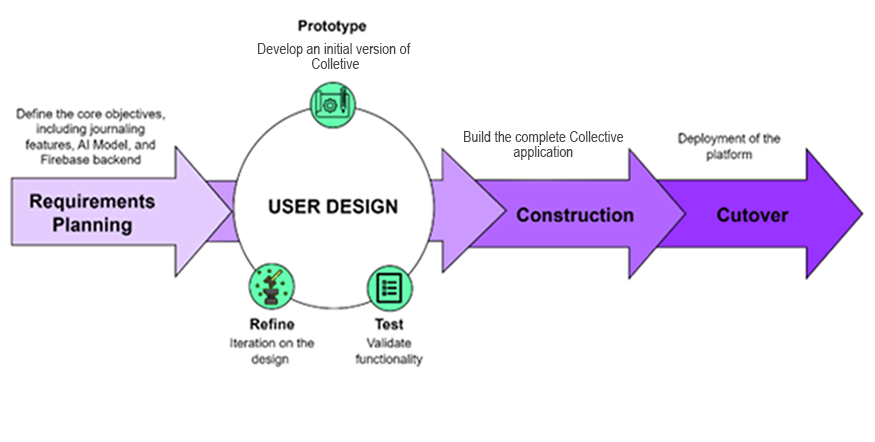
\includegraphics[width=0.8\textwidth]{files/imgs/RAD.png}
\caption{Rapid Application Development (RAD) Methodology Phases}
\label{fig:rad-methodology}
\end{figure}

Rapid Application Development (RAD) is a software development methodology that emphasizes quick development and iteration of prototypes over rigorous planning and testing. It is particularly useful for projects where requirements are expected to evolve or are not fully understood at the outset. The RAD methodology consists of four main phases: requirement planning, user design, construction, and cutover. This model was chosen for the development of the \textbf{Collective} mobile journaling application due to its flexibility and focus on user feedback, which is crucial for creating a user-friendly and effective application. The detais of the project is discussed below:

\section{Requirement planning}\label{sec:requirementPlanning}   

The requirement planning phase is the first step in the RAD methodology, where the project team identifies and defines the requirements of the application. This phase involves gathering information from stakeholders, including potential users, to understand their needs and expectations. The goal is to create a clear and concise set of requirements that will guide the development process.

\subsection{Software Requirements}\label{subsec:softwareRequirements}

The following tables list the software and tools used to develop the \textbf{Collective} mobile journaling application:

\begin{table}[H]
\centering
\caption{Visual Studio Code}
\label{tab:vscode-metadata}
\begin{tabular}{|p{4cm}|p{10cm}|}
\hline
\textbf{Attribute} & \textbf{Details} \\
\hline
Name & Visual Studio Code \\
\hline
Mnemonic & VS Code \\
\hline
Specification Number & N/A \\
\hline
Version Number & 1.101.1 \\
\hline
Source & \url{https://code.visualstudio.com/} \\
\hline
\end{tabular}
\end{table}

\begin{table}[H]
\centering
\caption{Flutter}
\label{tab:flutter-metadata}
\begin{tabular}{|p{4cm}|p{10cm}|}
\hline
\textbf{Attribute} & \textbf{Details} \\
\hline
Name & Flutter \\
\hline
Mnemonic & Flutter SDK \\
\hline
Specification Number & N/A \\
\hline
Version Number & 3.10.0 \\
\hline
Source & \url{https://flutter.dev/} \\
\hline
\end{tabular}
\end{table}

\begin{table}[H]
\centering
\caption{Dart}
\label{tab:dart-metadata}
\begin{tabular}{|p{4cm}|p{10cm}|}
\hline
\textbf{Attribute} & \textbf{Details} \\
\hline
Name & Dart \\
\hline
Mnemonic & Dart SDK \\
\hline
Specification Number & N/A \\
\hline
Version Number & 3.0.0 \\
\hline
Source & \url{https://dart.dev/} \\
\hline
\end{tabular}
\end{table}

\begin{table}[H]
\centering
\caption{Google Chrome}
\label{tab:chrome-metadata}
\begin{tabular}{|p{4cm}|p{10cm}|}
\hline
\textbf{Attribute} & \textbf{Details} \\
\hline
Name & Google Chrome \\
\hline
Mnemonic & Chrome Browser \\
\hline
Specification Number & N/A \\
\hline
Version Number & 114.0.5735.199 \\
\hline
Source & \url{https://www.google.com/chrome/} \\
\hline
\end{tabular}
\end{table}

\begin{table}[H]
\centering
\caption{Microsoft Word}
\label{tab:msword-metadata}
\begin{tabular}{|p{4cm}|p{10cm}|}
\hline
\textbf{Attribute} & \textbf{Details} \\
\hline
Name & Microsoft Word \\
\hline
Mnemonic & MS Word \\
\hline
Specification Number & N/A \\
\hline
Version Number & Office 365 \\
\hline
Source & \url{https://www.microsoft.com/en-us/microsoft-365/word} \\
\hline
\end{tabular}
\end{table}

\begin{table}[H]
\centering
\caption{Microsoft Excel}
\label{tab:msexcel-metadata}
\begin{tabular}{|p{4cm}|p{10cm}|}
\hline
\textbf{Attribute} & \textbf{Details} \\
\hline
Name & Microsoft Excel \\
\hline
Mnemonic & MS Excel \\
\hline
Specification Number & N/A \\
\hline
Version Number & Office 365 \\
\hline
Source & \url{https://www.microsoft.com/en-us/microsoft-365/excel} \\
\hline
\end{tabular}
\end{table}

\begin{table}[H]
\centering
\caption{Draw.io}
\label{tab:drawio-metadata}
\begin{tabular}{|p{4cm}|p{10cm}|}
\hline
\textbf{Attribute} & \textbf{Details} \\
\hline
Name & Draw.io \\
\hline
Mnemonic & Diagram Tool \\
\hline
Specification Number & N/A \\
\hline
Version Number & 20.8.0 \\
\hline
Source & \url{https://app.diagrams.net/} \\
\hline
\end{tabular}
\end{table}

\begin{table}[H]
\centering
\caption{DeepSeek API}
\label{tab:deepseek-metadata}
\begin{tabular}{|p{4cm}|p{10cm}|}
\hline
\textbf{Attribute} & \textbf{Details} \\
\hline
Name & DeepSeek API \\
\hline
Mnemonic & DeepSeek \\
\hline
Specification Number & N/A \\
\hline
Version Number & DeepSeek-V3-0324 \\
\hline
Source & \url{https://platform.deepseek.com/} \\
\hline
\end{tabular}
\end{table}

\subsection{Hardware Requirements}\label{subsec:hardwareRequirements}

The following table lists the hardware requirements necessary for the development and testing of the \textbf{Collective} mobile journaling application. Note that the development is currently focused exclusively on the Android platform, as iOS development requires a macOS machine, which is planned for future work:

\begin{table}[H]
\centering
\caption{Hardware Requirements}
\label{tab:hardware-requirements}
\begin{tabular}{|p{4cm}|p{10cm}|}
\hline
\textbf{Component} & \textbf{Specification} \\
\hline
Processor & Intel Core i5 or equivalent \\
\hline
RAM & 8 GB or higher \\
\hline
Storage & 256 GB SSD or higher \\
\hline
Operating System & Windows 10 \\
\hline
Additional Devices & Android smartphone for testing \\
\hline
\end{tabular}
\end{table}

\subsection{Use Case Diagram}\label{subsec:usecaseDiagram}

The use case diagram for the \textbf{Collective} mobile journaling application illustrates the interactions between the user (Writer) and the system. It highlights the various functionalities provided by the application and their relationships. The diagram is shown below:

\begin{figure}[H]
\centering
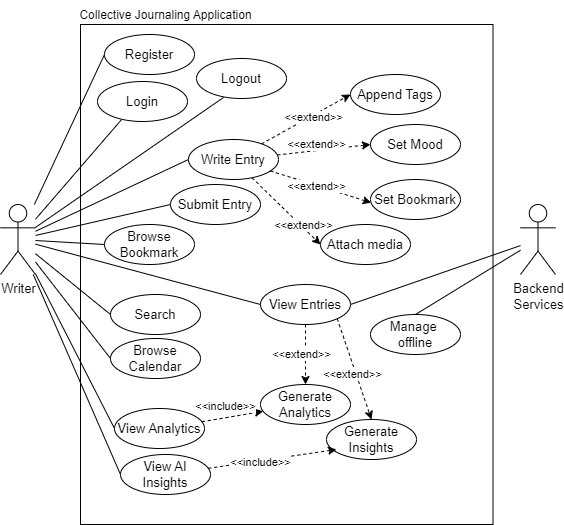
\includegraphics[width=0.8\textwidth]{files/imgs/usecase_diagram.png}
\caption{Use Case Diagram for Collective Mobile Journaling Application}
\label{fig:usecase-diagram}
\end{figure}

\subsection{Use Case Description}\label{subsec:usecaseDescription}

The use case description provides detailed information about the functionalities depicted in the use case diagram. Below is a table summarizing the key use cases:

\begin{table}[H]
\centering
\caption{Use Case Description}
\label{tab:usecase-description}
\begin{tabular}{|p{3cm}|p{5cm}|p{7cm}|}
\hline
\textbf{Actor} & \textbf{Use Case} & \textbf{Use Case Description} \\
\hline
\multirow{15}{*}{Writer} & Register & The writer can register their account by filling in their name, email, and password or use X or Google to register. \\
\cline{2-3}
 & Login & The writer can log in to the application using their registered credentials. \\
\cline{2-3}
 & Logout & The writer can log out of the application when they are done. \\
\cline{2-3}
 & Write Entry & The writer can compose journal entries to record their thoughts and experiences. \\
\cline{2-3}
 & Append Tags & The writer can add tags to their journal entries for better organization. \\
\cline{2-3}
 & Set Mood & The writer can set their mood for each journal entry to reflect their feelings. \\
\cline{2-3}
 & Set Bookmark & The writer can bookmark specific entries for quick access later. \\
\cline{2-3}
 & Attach Media & The writer can attach images or other media to their journal entries. \\
\cline{2-3}
 & Submit Entry & The writer can submit their journal entries to save them in the application. \\
\cline{2-3}
 & Browse Bookmark & The writer can browse through their bookmarked entries. \\
\cline{2-3}
 & View Entries & The writer can view all their saved journal entries. \\
\cline{2-3}
 & Search & The writer can search for specific entries using keywords. \\
\cline{2-3}
 & Browse Calendar & The writer can view their journal entries organized by calendar dates. \\
\cline{2-3}
 & View Analytics & The writer can analyze their journal entries to gain insights into their habits and patterns. \\
\cline{2-3}
 & View AI Insights & The writer can access AI-generated insights based on their journal entries. \\
\hline
\multirow{4}{*}{Backend Services} & View Entries & The system to store and retrieve the writer's journal entries securely. \\
\cline{2-3}
 & Manage Offline & The system to allow the writer to access their entries even when offline. \\
\cline{2-3}
 & Generate Analytics & The system to analyze the writer's journal entries to provide useful statistics. \\
\cline{2-3}
 & Generate Insights & The system to generate insights based on the writer's journal entries to help them understand their patterns. \\
\hline
\end{tabular}
\end{table}

\subsection{Constraints}\label{subsec:constraints}

This subsection outlines the genuine constraints that limit the development and operation of the Collective mobile journaling application.

\subsubsection{Development Constraints}

\textbf{Time Limitation:} As a final year project, development must be completed within one academic semester, limiting the scope of features that can be implemented and thoroughly tested.

\textbf{Single Developer:} The project is developed by one person, constraining the complexity of features and the amount of testing that can be performed across different scenarios and edge cases.

\textbf{Budget Limitation:} As a student project with no funding, all third-party services must use free tiers or minimal cost options, limiting AI processing capabilities and cloud storage quotas.

\subsubsection{Technical Constraints}

\textbf{AI Service Dependencies:} The application relies on external AI services (DeepSeek API) which impose rate limits and usage quotas, potentially limiting the frequency and depth of AI-powered insights.

\textbf{OAuth Provider Limitations:} Social authentication features depend on Google and Twitter/X OAuth services, which can change their policies or restrict access, potentially affecting user authentication options.

\subsubsection{Privacy and Legal Constraints}

\textbf{Data Sensitivity:} Journal entries contain highly personal information, requiring strict privacy protection measures and limiting data processing options to maintain user trust and legal compliance.

\textbf{Content Liability:} The private nature of journal entries means the system cannot implement automated content screening, creating potential liability concerns for harmful content.

\section{User design}\label{sec:userDesign}


The user design phase focuses on how users interact with the Collective application, shaping the interface and workflow based on user feedback and usability principles. This section details the main user roles and their interactions with the system, illustrated with activity diagrams for each core function.

\subsection{Process Flow}\label{subsec:processFlow}

\subsubsection{Writer}\label{subsubsec:writer}

The Writer is the primary user of the Collective application, responsible for creating, managing, and analyzing journal entries. The following functions are available to the Writer:

\textbf{i. Register}

Figure~\ref{fig:register-flow} shows the registration flow for new users. The writer can register using their email and password or authenticate through Google/X OAuth providers. The system validates the account details and, upon successful registration, redirects the writer to the journal screen where they can begin their journaling experience.

\begin{figure}[H]
\centering
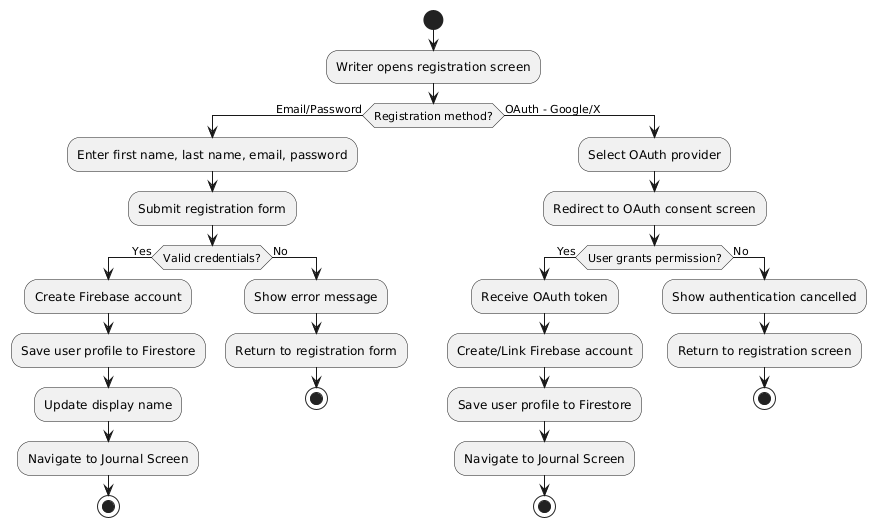
\includegraphics[width=0.95\textwidth,height=0.7\textheight,keepaspectratio]{files/imgs/register_flow.png}
\caption{Registration flow for Writer}
\label{fig:register-flow}
\end{figure}
\clearpage

\textbf{ii. Login}

Figure~\ref{fig:login-flow} shows the login flow for existing users. The writer can authenticate using their registered email and password or through their previously linked Google/X account. Upon successful authentication, the system validates the credentials and redirects the writer to the main journal screen.

\begin{figure}[H]
\centering
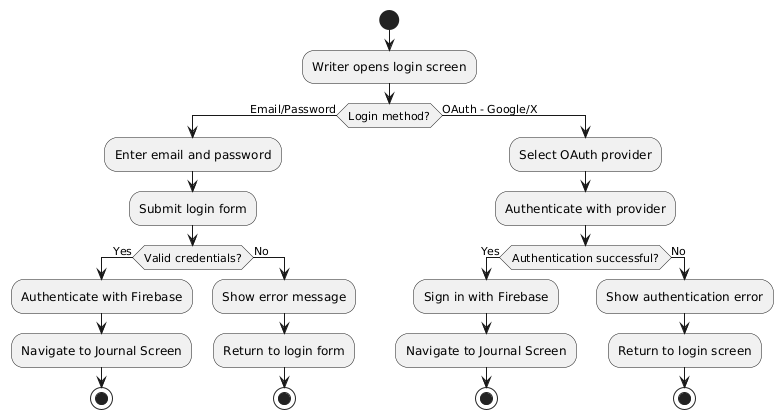
\includegraphics[width=0.95\textwidth,height=0.7\textheight,keepaspectratio]{files/imgs/login_flow.png}
\caption{Login flow for Writer}
\label{fig:login-flow}
\end{figure}
\clearpage

\textbf{iii. Write Entry}

Figure~\ref{fig:write-entry-flow} shows the entry creation flow for writers. The writer composes their journal entry in a distraction-free interface, optionally adds mood, tags, and media attachments, then saves the entry using the prominently displayed save button. The system processes the entry both locally and in the cloud when connectivity is available.

\begin{figure}[H]
\centering
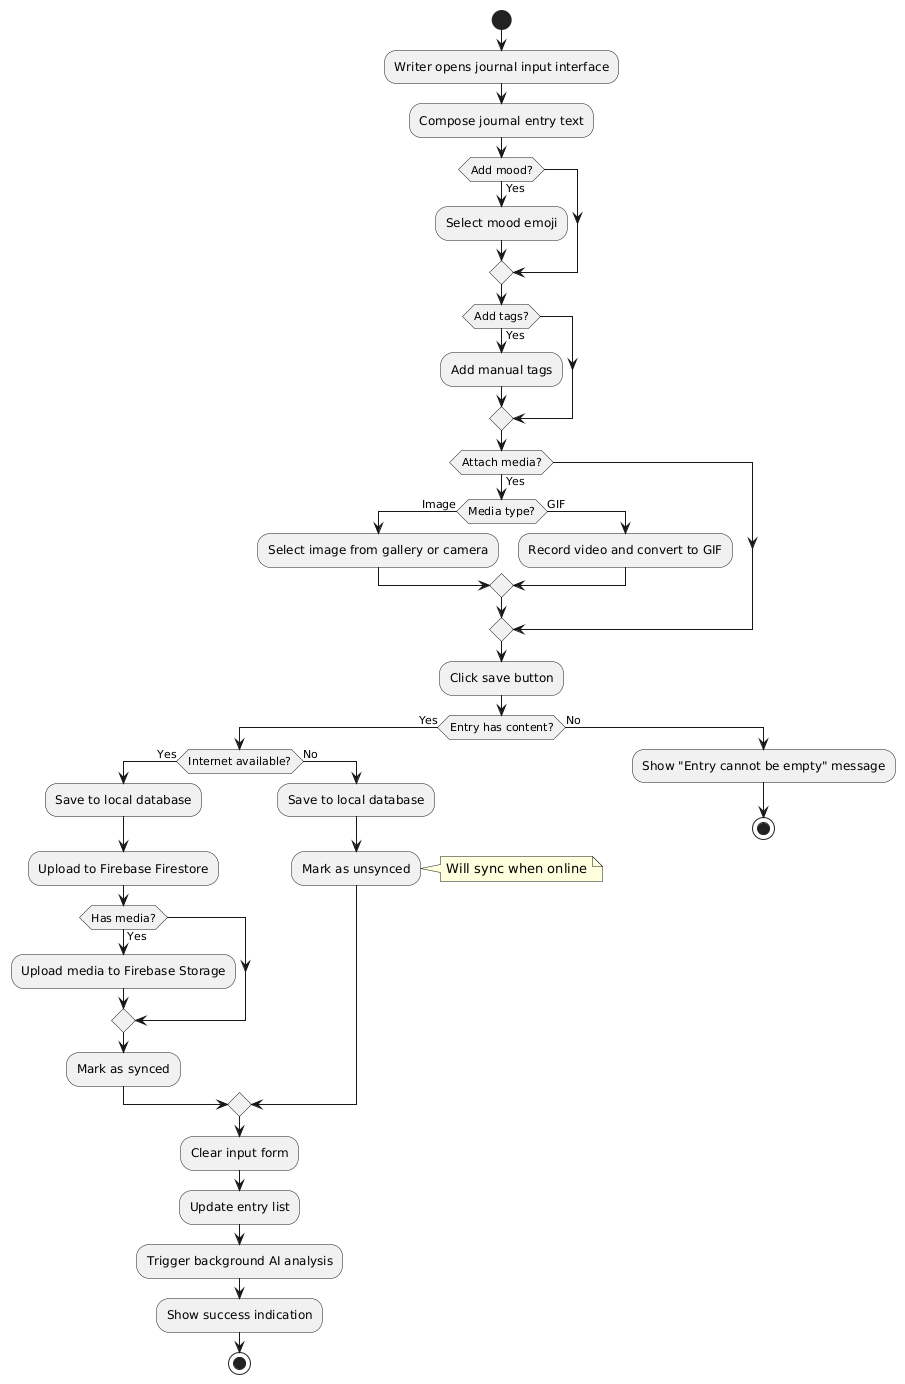
\includegraphics[width=0.95\textwidth,height=0.7\textheight,keepaspectratio]{files/imgs/write_entry_flow.png}
\caption{Write Entry flow for Writer}
\label{fig:write-entry-flow}
\end{figure}
\clearpage

\textbf{iv. Edit Entry}

Figure~\ref{fig:edit-entry-flow} shows the entry editing flow for writers. The writer can modify existing entries, update their mood, change tags, or replace media attachments. The system tracks changes and updates both local and cloud storage accordingly.

\begin{figure}[H]
\centering
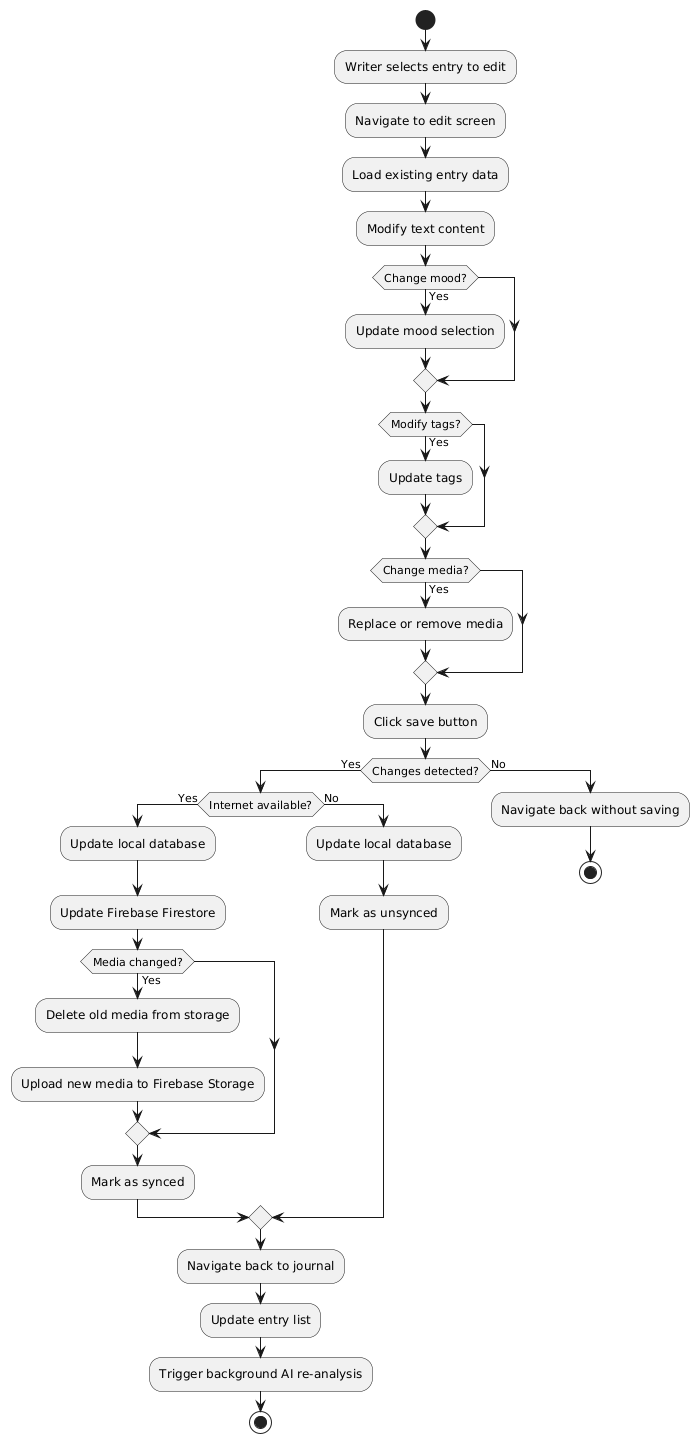
\includegraphics[width=0.95\textwidth,height=0.7\textheight,keepaspectratio]{files/imgs/edit_entry_flow.png}
\caption{Edit Entry flow for Writer}
\label{fig:edit-entry-flow}
\end{figure}
\clearpage

\textbf{v. Search}

Figure~\ref{fig:search-flow} shows the search functionality flow. The writer can search through their entries using fuzzy search algorithms that match both entry content and tags, providing intelligent search results even with partial or approximate queries.

\begin{figure}[H]
\centering
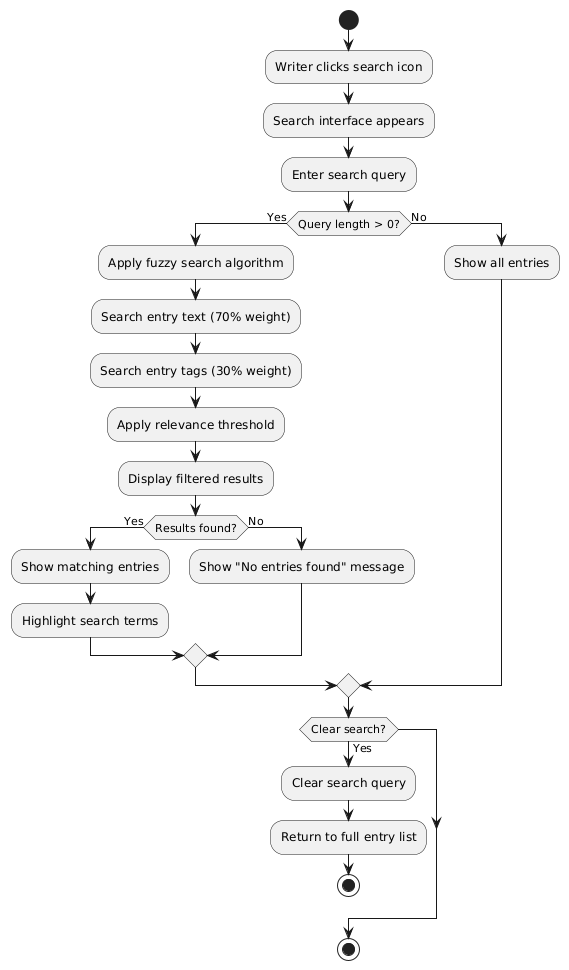
\includegraphics[width=0.95\textwidth,height=0.7\textheight,keepaspectratio]{files/imgs/search_flow.png}
\caption{Search flow for Writer}
\label{fig:search-flow}
\end{figure}
\clearpage

\textbf{vi. Analytics}

Figure~\ref{fig:analytics-flow} shows the analytics viewing flow. The writer can access AI-generated insights about their journaling patterns, emotional trends, and topic clusters. The system uses cached analytics data when available and generates new analysis when needed.

\begin{figure}[H]
\centering
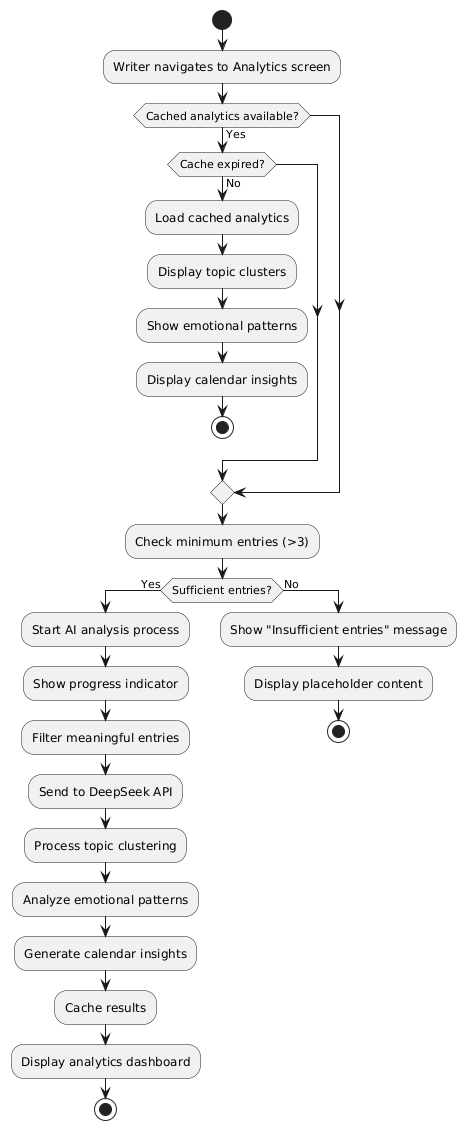
\includegraphics[width=0.95\textwidth,height=0.7\textheight,keepaspectratio]{files/imgs/analytics_flow.png}
\caption{Analytics flow for Writer}
\label{fig:analytics-flow}
\end{figure}
\clearpage

\textbf{vii. Insights}

Figure~\ref{fig:insights-flow} shows the AI insights viewing flow for individual entries. The writer can access detailed analysis of specific entries, including contextual relationships, emotional analysis, and personalized recommendations.

\begin{figure}[H]
\centering
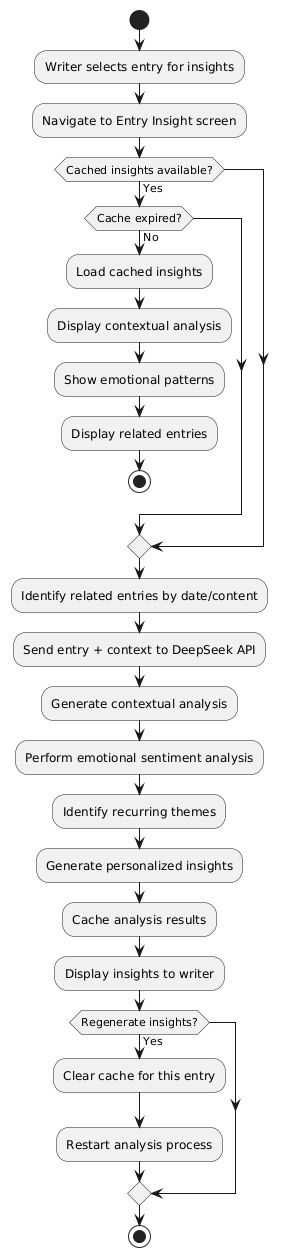
\includegraphics[width=0.95\textwidth,height=0.7\textheight,keepaspectratio]{files/imgs/insights_flow.png}
\caption{Insights flow for Writer}
\label{fig:insights-flow}
\end{figure}
\clearpage

\textbf{viii. Logout}

Figure~\ref{fig:logout-flow} shows the logout process for writers. The system securely terminates the user session, clears authentication tokens, and redirects to the login screen while ensuring local data remains protected.

\begin{figure}[H]
\centering
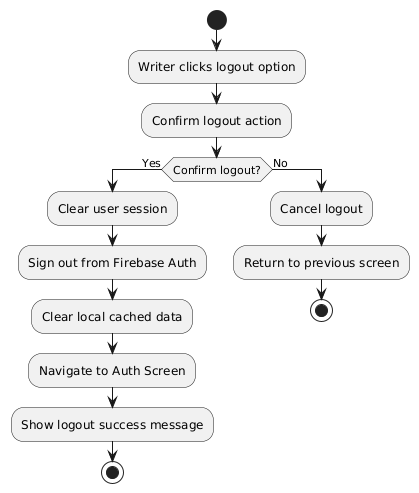
\includegraphics[width=0.95\textwidth,height=0.7\textheight,keepaspectratio]{files/imgs/logout_flow.png}
\caption{Logout flow for Writer}
\label{fig:logout-flow}
\end{figure}
\clearpage

\textbf{ix. Append Tags}

Figure~\ref{fig:append-tags-flow} shows the tag management flow. Writers can add, modify, or remove tags from their entries to improve organization and searchability. The system provides tag suggestions based on entry content and previous usage patterns.

\begin{figure}[H]
\centering
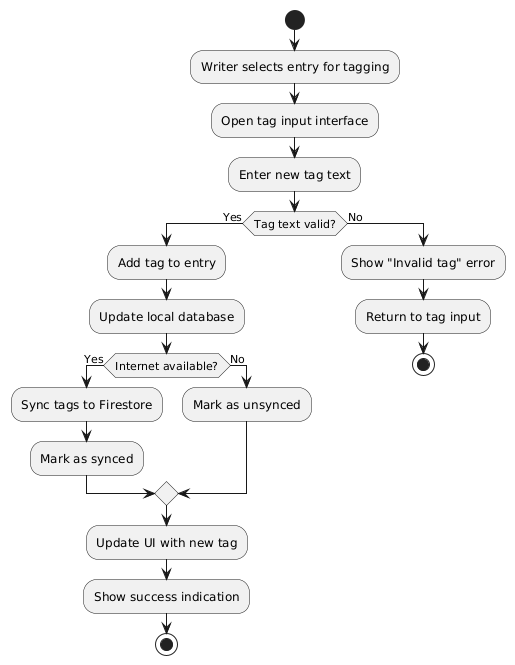
\includegraphics[width=0.95\textwidth,height=0.7\textheight,keepaspectratio]{files/imgs/append_tags_flow.png}
\caption{Append Tags flow for Writer}
\label{fig:append-tags-flow}
\end{figure}
\clearpage

\textbf{x. Set Mood}

Figure~\ref{fig:set-mood-flow} shows the mood setting functionality. Writers can associate emotional states with their entries, enabling the system to track emotional patterns over time and provide relevant insights.

\begin{figure}[H]
\centering
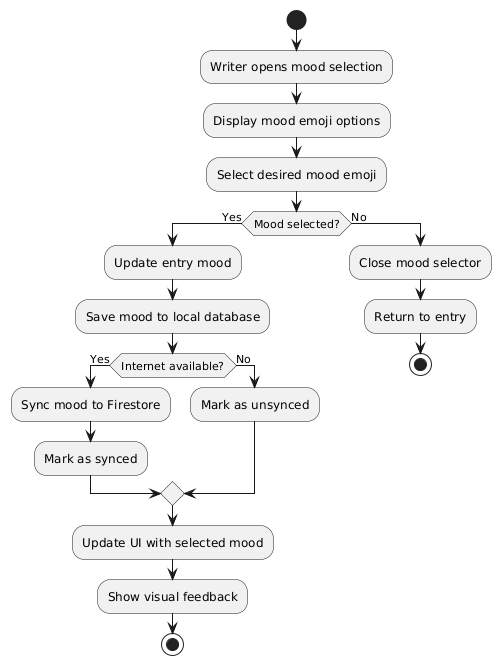
\includegraphics[width=0.95\textwidth,height=0.7\textheight,keepaspectratio]{files/imgs/set_mood_flow.png}
\caption{Set Mood flow for Writer}
\label{fig:set-mood-flow}
\end{figure}
\clearpage

\textbf{xi. Set Bookmark}

Figure~\ref{fig:set-bookmark-flow} shows the bookmarking process. Writers can mark important entries for quick access, creating a personalized collection of significant journal entries.

\begin{figure}[H]
\centering
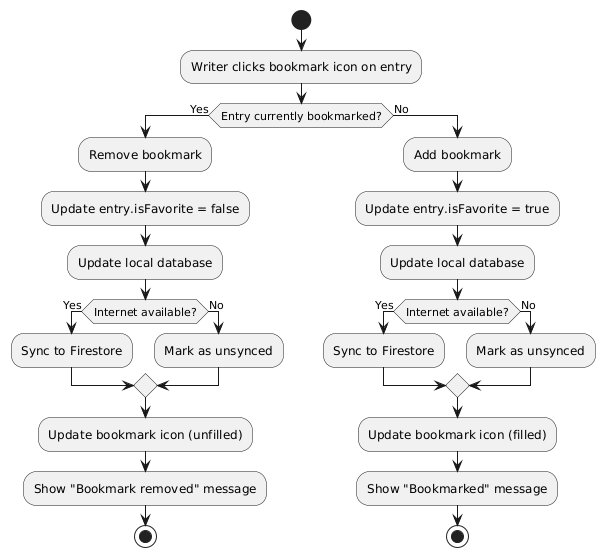
\includegraphics[width=0.95\textwidth,height=0.7\textheight,keepaspectratio]{files/imgs/set_bookmark_flow.png}
\caption{Set Bookmark flow for Writer}
\label{fig:set-bookmark-flow}
\end{figure}
\clearpage

\textbf{xii. Attach Media}

Figure~\ref{fig:attach-media-flow} shows the media attachment process. Writers can enhance their entries with images, GIFs, or other media content, with the system handling compression and storage optimization automatically.

\begin{figure}[H]
\centering
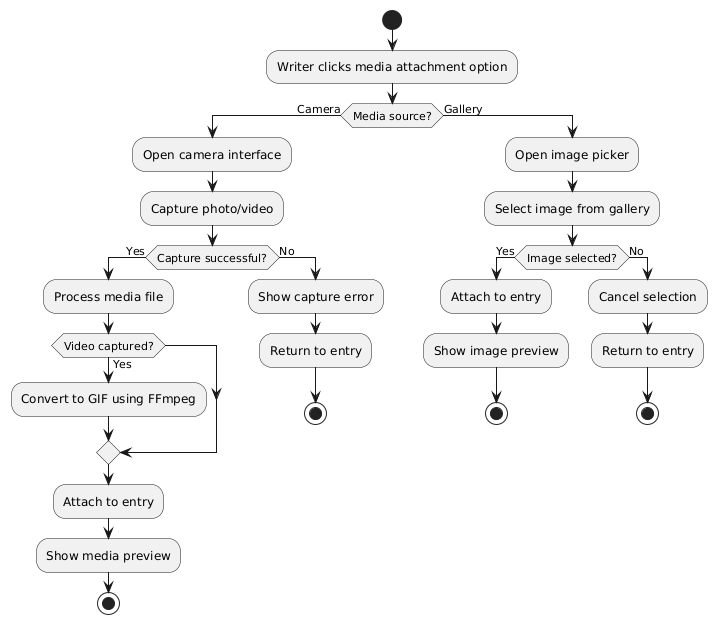
\includegraphics[width=0.95\textwidth,height=0.7\textheight,keepaspectratio]{files/imgs/attach_media_flow.png}
\caption{Attach Media flow for Writer}
\label{fig:attach-media-flow}
\end{figure}
\clearpage

\textbf{xiii. Browse Bookmark}

Figure~\ref{fig:browse-bookmark-flow} shows the bookmark browsing functionality. Writers can efficiently navigate through their bookmarked entries, with options for sorting and filtering based on various criteria.

\begin{figure}[H]
\centering
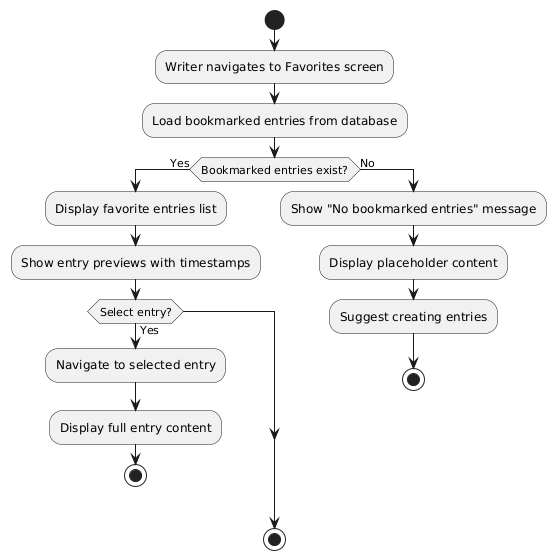
\includegraphics[width=0.95\textwidth,height=0.7\textheight,keepaspectratio]{files/imgs/browse_bookmark_flow.png}
\caption{Browse Bookmark flow for Writer}
\label{fig:browse-bookmark-flow}
\end{figure}
\clearpage

\textbf{xiv. View Entries}

Figure~\ref{fig:view-entries-flow} shows the entry viewing interface. Writers can browse through all their journal entries with various viewing options including list view, timeline view, and calendar integration.

\begin{figure}[H]
\centering
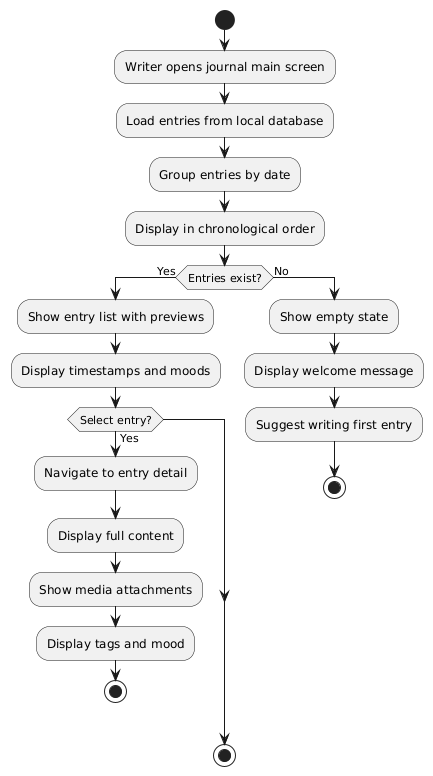
\includegraphics[width=0.95\textwidth,height=0.7\textheight,keepaspectratio]{files/imgs/view_entries_flow.png}
\caption{View Entries flow for Writer}
\label{fig:view-entries-flow}
\end{figure}
\clearpage

\textbf{xv. Browse Calendar}

Figure~\ref{fig:browse-calendar-flow} shows the calendar browsing functionality. Writers can navigate through their journaling history using an intuitive calendar interface, quickly jumping to entries from specific dates.

\begin{figure}[H]
\centering
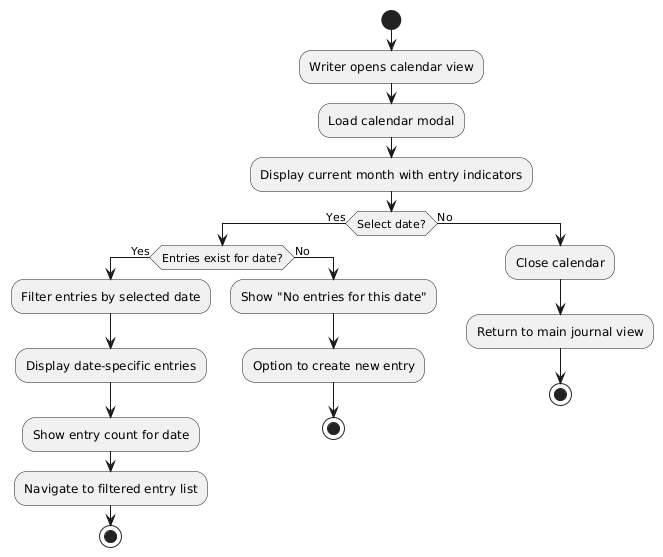
\includegraphics[width=0.95\textwidth,height=0.7\textheight,keepaspectratio]{files/imgs/browse_calendar_flow.png}
\caption{Browse Calendar flow for Writer}
\label{fig:browse-calendar-flow}
\end{figure}
\clearpage

\subsubsection{Backend Services}\label{subsubsec:backendServices}

This subsection covers the backend functionalities that support the user-facing features, including data management, synchronization, and AI processing capabilities.

\textbf{i. Store/Retrieve Entries}

Figure~\ref{fig:store-retrieve-entries-flow} shows the data management process for journal entries. The system handles secure storage and retrieval of entries across local and cloud storage, ensuring data integrity and availability.

\begin{figure}[H]
\centering
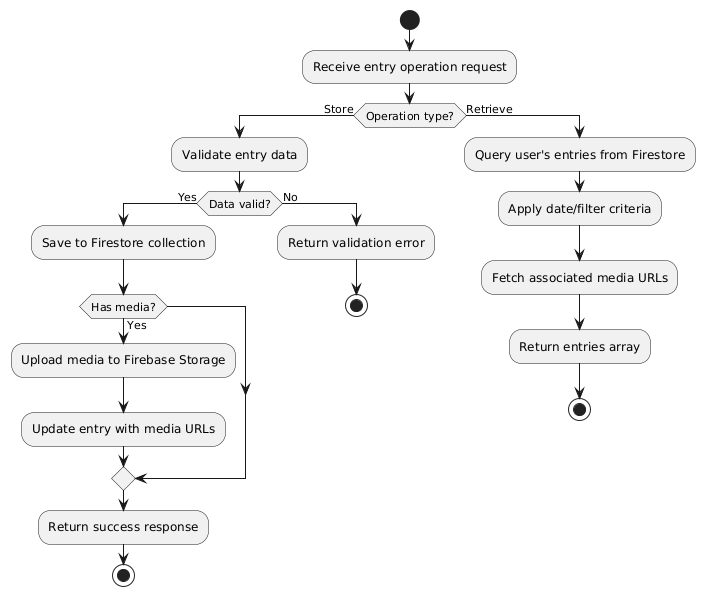
\includegraphics[width=0.8\textwidth]{files/imgs/store_retrieve_entries_flow.png}
\caption{Store/Retrieve Entries Flow}
\label{fig:store-retrieve-entries-flow}
\end{figure}
\clearpage

\textbf{ii. Manage Offline}

Figure~\ref{fig:manage-offline-flow} shows the offline functionality management. The system automatically handles offline mode, local data storage, and synchronization when connectivity is restored, ensuring seamless user experience regardless of network availability.

\begin{figure}[H]
\centering
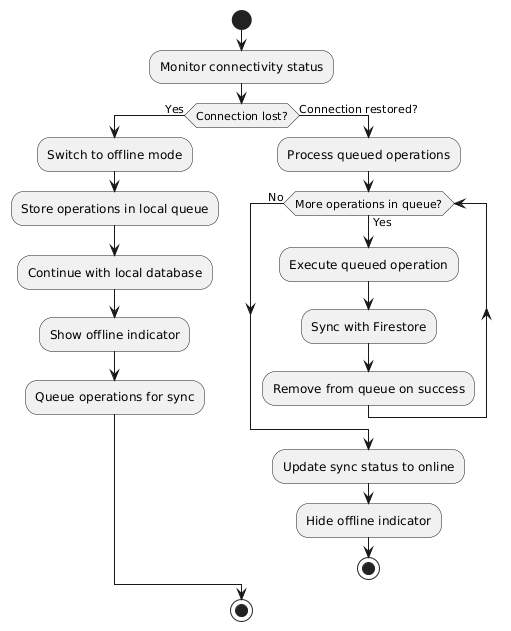
\includegraphics[width=0.8\textwidth]{files/imgs/manage_offline_flow.png}
\caption{Manage Offline Flow}
\label{fig:manage-offline-flow}
\end{figure}
\clearpage

\textbf{iii. Sync}

Figure~\ref{fig:sync-flow} shows the synchronization process between local and cloud storage. The system automatically detects connectivity changes and synchronizes data when internet access is available, maintaining data consistency across devices.

\begin{figure}[H]
\centering
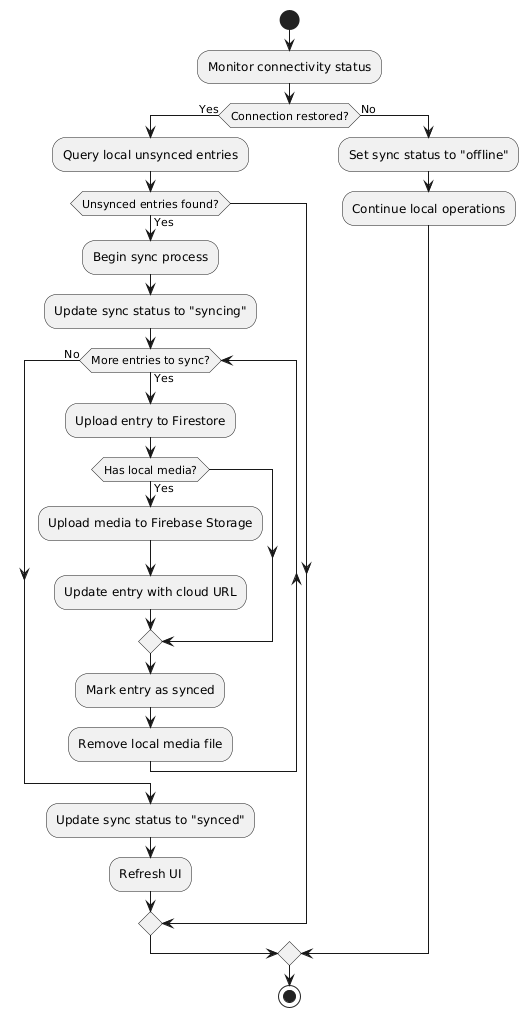
\includegraphics[width=0.95\textwidth,height=0.7\textheight,keepaspectratio]{files/imgs/sync_flow.png}
\caption{Synchronization Flow}
\label{fig:sync-flow}
\end{figure}
\clearpage

\textbf{iv. AI Processing}

Figure~\ref{fig:ai-processing-flow} shows the background AI processing that occurs automatically after entries are saved. The system performs sentiment analysis, pattern recognition, and insight generation without user intervention to maintain the simplicity of the journaling experience.

\begin{figure}[H]
\centering
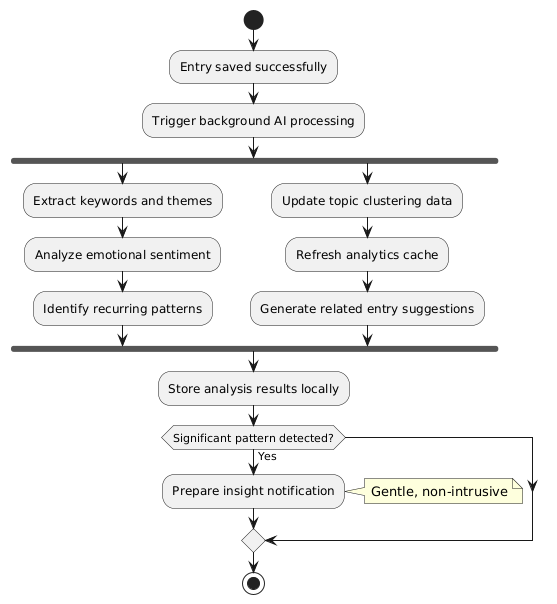
\includegraphics[width=0.8\textwidth]{files/imgs/ai_processing_flow.png}
\caption{AI Processing Flow}
\label{fig:ai-processing-flow}
\end{figure}
\clearpage

\subsection{Use Case}\label{subsec:useCase}

This subsection presents detailed use case analysis for the Collective mobile journaling application. Each use case includes a visual UML diagram and detailed specification table covering the use case ID, name, purpose, role, and various scenarios. The use cases are organized by functionality and provide comprehensive coverage of all system features available to writers.

\subsubsection{Register}

Figure~\ref{fig:usecase-register} shows the register use case diagram. This use case allows new users to create an account using email/password credentials or through OAuth providers like Google and Twitter/X.

\begin{figure}[H]
\centering
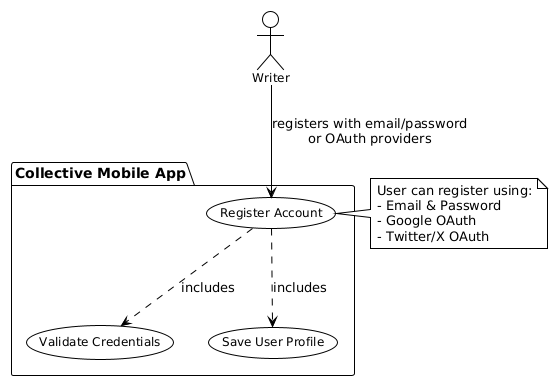
\includegraphics[width=0.8\textwidth]{files/imgs/usecase_U9ojKajF0Z.png}
\caption{Use Case Register}
\label{fig:usecase-register}
\end{figure}

\begin{table}[H]
\centering
\caption{Use Case Register Details}
\label{tab:usecase-register}
\begin{tabular}{|p{3cm}|p{11cm}|}
\hline
\textbf{Use Case ID} & UC-001 \\
\hline
\textbf{Use Case Name} & Register \\
\hline
\textbf{Purpose} & To allow writers to register a new account in the Collective application \\
\hline
\textbf{Role} & Writers \\
\hline
\textbf{Base Scenario} & 1. Writer opens the application for the first time \newline 2. Writer selects registration option \newline 3. Writer enters first name, last name, email, and password \newline 4. System validates the provided information \newline 5. System creates user profile in Firebase \newline 6. Writer is redirected to the main journal screen \\
\hline
\textbf{Alternative Scenario} & 1. Writer selects Google OAuth registration \newline 2. System redirects to Google authentication \newline 3. Writer authorizes the application \newline 4. System creates user profile using Google information \newline OR \newline 1. Writer selects Twitter/X OAuth registration \newline 2. System redirects to Twitter authentication \newline 3. Writer authorizes the application \newline 4. System creates user profile using Twitter information \\
\hline
\textbf{Exception Scenario} & 1. Email already exists in the system - System displays error message \newline 2. Invalid email format - System displays validation error \newline 3. Weak password - System requests stronger password \newline 4. Network connectivity issues - System displays retry option \newline 5. OAuth provider unavailable - System falls back to email registration \\
\hline
\end{tabular}
\end{table}

\subsubsection{Login}

Figure~\ref{fig:usecase-login} shows the login use case diagram. This use case enables existing users to authenticate and access their journal entries.

\begin{figure}[H]
\centering
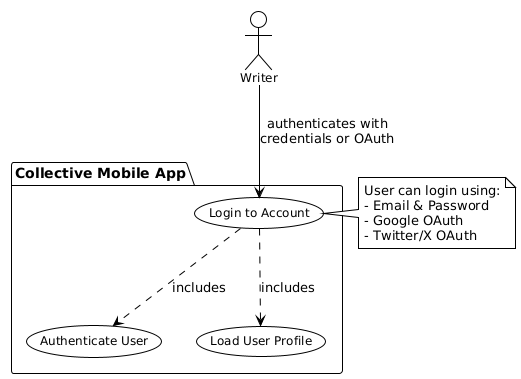
\includegraphics[width=0.8\textwidth]{files/imgs/usecase_U9ojKZrFmp.png}
\caption{Use Case Login}
\label{fig:usecase-login}
\end{figure}

\begin{table}[H]
\centering
\caption{Use Case Login Details}
\label{tab:usecase-login}
\begin{tabular}{|p{3cm}|p{11cm}|}
\hline
\textbf{Use Case ID} & UC-002 \\
\hline
\textbf{Use Case Name} & Login \\
\hline
\textbf{Purpose} & To allow writers to login into their existing account \\
\hline
\textbf{Role} & Writers \\
\hline
\textbf{Base Scenario} & 1. Writer opens the application \newline 2. Writer enters registered email and password \newline 3. System validates credentials against Firebase Authentication \newline 4. System loads user profile and preferences \newline 5. Writer is redirected to the main journal screen with access to their entries \\
\hline
\textbf{Alternative Scenario} & 1. Writer selects Google OAuth login \newline 2. System authenticates with Google services \newline 3. System validates existing account \newline 4. Writer gains immediate access to their journal \newline OR \newline 1. Writer selects Twitter/X OAuth login \newline 2. System authenticates with Twitter services \newline 3. System validates existing account \newline 4. Writer gains immediate access to their journal \\
\hline
\textbf{Exception Scenario} & 1. Incorrect email or password - System displays authentication error \newline 2. Account not found - System suggests registration \newline 3. Account temporarily locked - System displays wait message \newline 4. Network connectivity issues - System enables offline mode \newline 5. OAuth provider authentication fails - System provides alternative login methods \\
\hline
\end{tabular}
\end{table}

\subsubsection{Logout}

Figure~\ref{fig:usecase-logout} shows the logout use case diagram. This use case allows writers to securely terminate their session.

\begin{figure}[H]
\centering
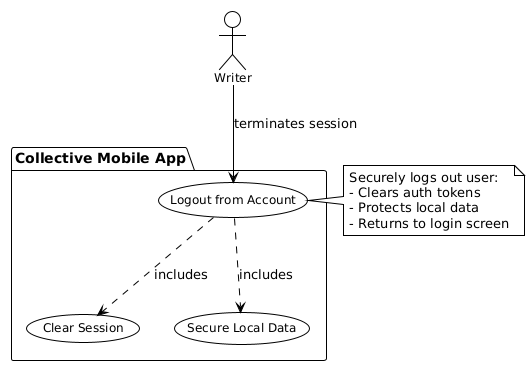
\includegraphics[width=0.8\textwidth]{files/imgs/usecase_U9ojaazFmp.png}
\caption{Use Case Logout}
\label{fig:usecase-logout}
\end{figure}

\begin{table}[H]
\centering
\caption{Use Case Logout Details}
\label{tab:usecase-logout}
\begin{tabular}{|p{3cm}|p{11cm}|}
\hline
\textbf{Use Case ID} & UC-003 \\
\hline
\textbf{Use Case Name} & Logout \\
\hline
\textbf{Purpose} & To allow writers to securely logout from their account \\
\hline
\textbf{Role} & Writers \\
\hline
\textbf{Base Scenario} & 1. Writer accesses logout option from the application menu \newline 2. System confirms logout intent \newline 3. System clears authentication tokens and session data \newline 4. System secures local data storage \newline 5. Writer is redirected to the login screen \\
\hline
\textbf{Alternative Scenario} & 1. Automatic logout due to session expiry \newline 2. System automatically clears session \newline 3. System displays session timeout message \newline 4. Writer is redirected to login screen \\
\hline
\textbf{Exception Scenario} & 1. Network issues during logout - System performs local logout and attempts sync later \newline 2. Unsaved data exists - System prompts to save before logout \newline 3. System error during logout - System forces local session termination \\
\hline
\end{tabular}
\end{table}

\subsubsection{Write Entry}

Figure~\ref{fig:usecase-write-entry} shows the write entry use case diagram. This core functionality allows writers to create new journal entries.

\begin{figure}[H]
\centering
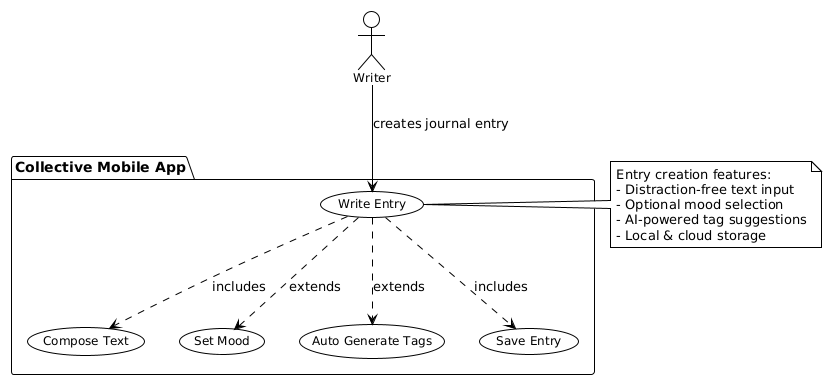
\includegraphics[width=0.8\textwidth]{files/imgs/usecase_U9ojKZjFmp.png}
\caption{Use Case Write Entry}
\label{fig:usecase-write-entry}
\end{figure}

\begin{table}[H]
\centering
\caption{Use Case Write Entry Details}
\label{tab:usecase-write-entry}
\begin{tabular}{|p{3cm}|p{11cm}|}
\hline
\textbf{Use Case ID} & UC-004 \\
\hline
\textbf{Use Case Name} & Write Entry \\
\hline
\textbf{Purpose} & To allow writers to create new journal entries with text, mood, and optional media \\
\hline
\textbf{Role} & Writers \\
\hline
\textbf{Base Scenario} & 1. Writer opens the journal input interface \newline 2. Writer composes their thoughts in the text area \newline 3. Writer optionally selects a mood from predefined options \newline 4. Writer optionally adds tags for organization \newline 5. Writer saves the entry using the save action \newline 6. System stores entry locally and syncs to cloud when available \\
\hline
\textbf{Alternative Scenario} & 1. Writer attaches an image to the entry \newline 2. System compresses and optimizes the media \newline 3. Writer continues with text composition \newline 4. System saves entry with media attachment \newline OR \newline 1. Writer creates entry while offline \newline 2. System saves entry to local database \newline 3. System queues entry for cloud sync when connectivity returns \\
\hline
\textbf{Exception Scenario} & 1. Empty entry attempted - System displays validation message \newline 2. Network failure during save - System saves locally and retries sync \newline 3. Storage space insufficient - System alerts user and suggests cleanup \newline 4. Image attachment too large - System compresses or requests smaller file \\
\hline
\end{tabular}
\end{table}

\subsubsection{Append Tags}

Figure~\ref{fig:usecase-append-tags} shows the append tags use case diagram. This functionality helps organize entries through tagging.

\begin{figure}[H]
\centering
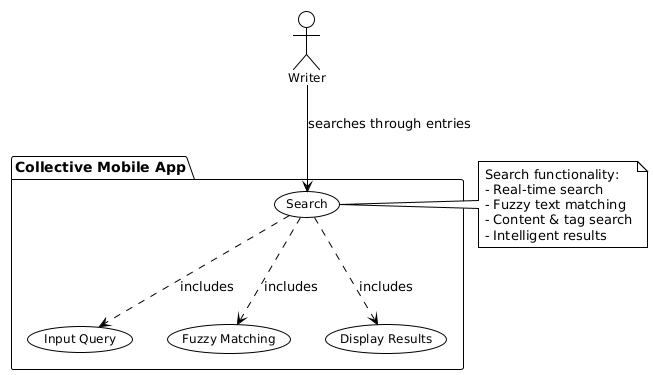
\includegraphics[width=0.8\textwidth]{files/imgs/usecase_U9ojKh5kmZ.png}
\caption{Use Case Append Tags}
\label{fig:usecase-append-tags}
\end{figure}

\begin{table}[H]
\centering
\caption{Use Case Append Tags Details}
\label{tab:usecase-append-tags}
\begin{tabular}{|p{3cm}|p{11cm}|}
\hline
\textbf{Use Case ID} & UC-005 \\
\hline
\textbf{Use Case Name} & Append Tags \\
\hline
\textbf{Purpose} & To allow writers to add organizational tags to their journal entries \\
\hline
\textbf{Role} & Writers \\
\hline
\textbf{Base Scenario} & 1. Writer accesses tag management for an entry \newline 2. System displays existing tags and suggestions \newline 3. Writer selects from suggested tags or creates custom tags \newline 4. Writer applies tags to the entry \newline 5. System updates entry metadata and improves future suggestions \\
\hline
\textbf{Alternative Scenario} & 1. AI system analyzes entry content \newline 2. System automatically suggests relevant tags \newline 3. Writer reviews and accepts/modifies suggestions \newline 4. System learns from writer preferences for future entries \\
\hline
\end{tabular}
\end{table}

\subsubsection{Set Mood}

Figure~\ref{fig:usecase-set-mood} shows the set mood use case diagram. This feature enables emotional tracking within entries.

\begin{figure}[H]
\centering
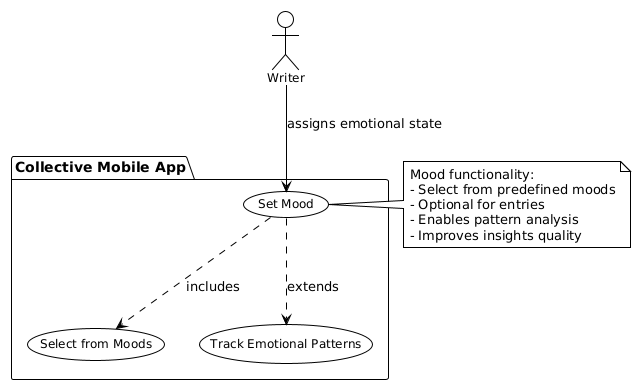
\includegraphics[width=0.8\textwidth]{files/imgs/usecase_U9ojKarFma.png}
\caption{Use Case Set Mood}
\label{fig:usecase-set-mood}
\end{figure}

\begin{table}[H]
\centering
\caption{Use Case Set Mood Details}
\label{tab:usecase-set-mood}
\begin{tabular}{|p{3cm}|p{11cm}|}
\hline
\textbf{Use Case ID} & UC-006 \\
\hline
\textbf{Use Case Name} & Set Mood \\
\hline
\textbf{Purpose} & To allow writers to associate emotional states with their journal entries \\
\hline
\textbf{Role} & Writers \\
\hline
\textbf{Base Scenario} & 1. Writer accesses mood selection interface during entry creation \newline 2. System displays predefined mood options (happy, sad, anxious, etc.) \newline 3. Writer selects the mood that best represents their emotional state \newline 4. System associates the mood with the entry for pattern analysis \newline 5. System updates emotional tracking data for analytics \\
\hline
\textbf{Alternative Scenario} & 1. Writer chooses not to set a mood (optional feature) \newline 2. System saves entry without mood association \newline 3. Entry remains available for mood addition later \newline OR \newline 1. Writer changes mood after initial entry creation \newline 2. System updates mood association \newline 3. System recalculates emotional patterns if needed \\
\hline
\textbf{Exception Scenario} & 1. Mood data inconsistency - System uses default neutral mood \newline 2. Multiple mood selections attempted - System uses last selection \newline 3. Invalid mood data - System prompts for re-selection \\
\hline
\end{tabular}
\end{table}

\subsubsection{Set Bookmark}

Figure~\ref{fig:usecase-set-bookmark} shows the set bookmark use case diagram. This feature allows writers to mark important entries.

\begin{figure}[H]
\centering
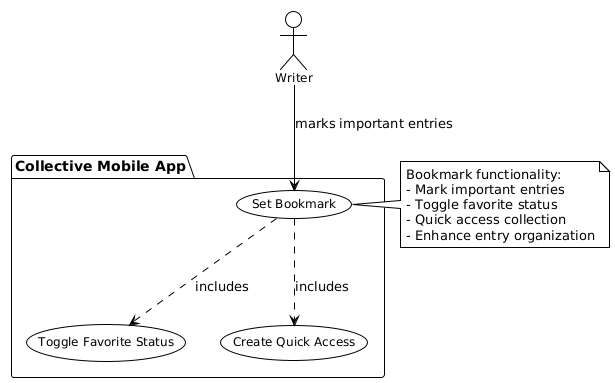
\includegraphics[width=0.8\textwidth]{files/imgs/usecase_U9ojaZzlWp.png}
\caption{Use Case Set Bookmark}
\label{fig:usecase-set-bookmark}
\end{figure}

\begin{table}[H]
\centering
\caption{Use Case Set Bookmark Details}
\label{tab:usecase-set-bookmark}
\begin{tabular}{|p{3cm}|p{11cm}|}
\hline
\textbf{Use Case ID} & UC-007 \\
\hline
\textbf{Use Case Name} & Set Bookmark \\
\hline
\textbf{Purpose} & To allow writers to bookmark important entries for quick access \\
\hline
\textbf{Role} & Writers \\
\hline
\textbf{Base Scenario} & 1. Writer identifies an important entry to bookmark \newline 2. Writer selects the bookmark/favorite option \newline 3. System toggles the bookmark status of the entry \newline 4. System updates the entry metadata \newline 5. Entry becomes accessible through the favorites collection \\
\hline
\textbf{Alternative Scenario} & 1. Writer removes bookmark from previously bookmarked entry \newline 2. System toggles bookmark status to off \newline 3. Entry is removed from favorites collection but remains in main timeline \\
\hline
\textbf{Exception Scenario} & 1. Bookmark data corruption - System resets bookmark status \newline 2. Sync conflict with bookmark status - System uses most recent version \newline 3. Maximum bookmarks reached - System displays limit notification \\
\hline
\end{tabular}
\end{table}

\subsubsection{Attach Media}

Figure~\ref{fig:usecase-attach-media} shows the attach media use case diagram. This functionality enhances entries with visual content.

\begin{figure}[H]
\centering
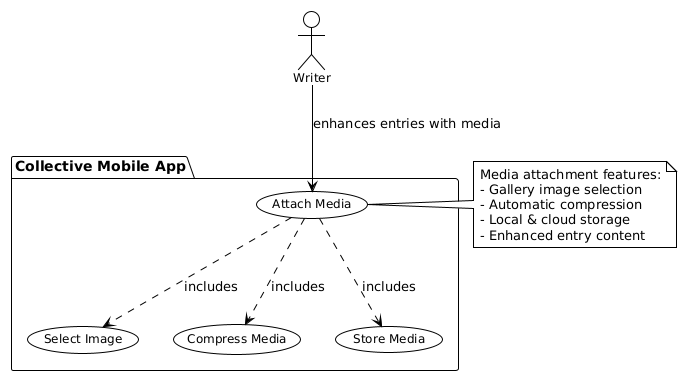
\includegraphics[width=0.8\textwidth]{files/imgs/usecase_U9ojKZjhmp.png}
\caption{Use Case Attach Media}
\label{fig:usecase-attach-media}
\end{figure}

\begin{table}[H]
\centering
\caption{Use Case Attach Media Details}
\label{tab:usecase-attach-media}
\begin{tabular}{|p{3cm}|p{11cm}|}
\hline
\textbf{Use Case ID} & UC-008 \\
\hline
\textbf{Use Case Name} & Attach Media \\
\hline
\textbf{Purpose} & To allow writers to enhance their entries with images and media content \\
\hline
\textbf{Role} & Writers \\
\hline
\textbf{Base Scenario} & 1. Writer selects media attachment option during entry creation \newline 2. System opens device gallery or camera interface \newline 3. Writer selects or captures an image \newline 4. System compresses and optimizes the media file \newline 5. System associates media with the entry and stores locally \newline 6. System uploads media to cloud storage when connectivity available \\
\hline
\textbf{Alternative Scenario} & 1. Writer attaches multiple images to single entry \newline 2. System processes each image individually \newline 3. System creates media gallery for the entry \newline OR \newline 1. Writer removes attached media \newline 2. System removes media association and files \newline 3. System updates entry metadata \\
\hline
\textbf{Exception Scenario} & 1. Image file too large - System compresses or requests smaller file \newline 2. Unsupported file format - System displays supported format message \newline 3. Storage space insufficient - System alerts and suggests cleanup \newline 4. Upload failure - System retries upload when connectivity restored \newline 5. Corrupted media file - System displays error and removes attachment \\
\hline
\end{tabular}
\end{table}

\subsubsection{Submit Entry}

Figure~\ref{fig:usecase-submit-entry} shows the submit entry use case diagram. This finalizes the entry creation process.

\begin{figure}[H]
\centering
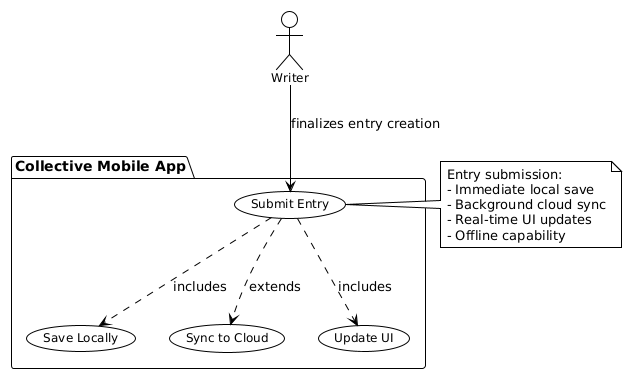
\includegraphics[width=0.8\textwidth]{files/imgs/usecase_U9ojaa5Fmp.png}
\caption{Use Case Submit Entry}
\label{fig:usecase-submit-entry}
\end{figure}

\begin{table}[H]
\centering
\caption{Use Case Submit Entry Details}
\label{tab:usecase-submit-entry}
\begin{tabular}{|p{3cm}|p{11cm}|}
\hline
\textbf{Use Case ID} & UC-009 \\
\hline
\textbf{Use Case Name} & Submit Entry \\
\hline
\textbf{Purpose} & To allow writers to finalize and save their completed journal entries \\
\hline
\textbf{Role} & Writers \\
\hline
\textbf{Base Scenario} & 1. Writer completes entry composition with text, mood, tags, and media \newline 2. Writer selects save/submit action \newline 3. System validates entry content and metadata \newline 4. System saves entry to local database immediately \newline 5. System updates UI to reflect new entry \newline 6. System queues entry for cloud synchronization \\
\hline
\textbf{Alternative Scenario} & 1. Auto-save triggers during entry composition \newline 2. System saves draft entry periodically \newline 3. Writer can continue editing or finalize submission \newline OR \newline 1. Writer submits entry while offline \newline 2. System saves locally with sync pending status \newline 3. System syncs when connectivity restored \\
\hline
\textbf{Exception Scenario} & 1. Entry validation fails - System highlights issues and prevents submission \newline 2. Local storage full - System displays storage warning \newline 3. Duplicate entry detected - System asks for confirmation \newline 4. System crash during submission - System recovers draft on restart \\
\hline
\end{tabular}
\end{table}

\subsubsection{Browse Bookmark}

Figure~\ref{fig:usecase-browse-bookmark} shows the browse bookmark use case diagram. This provides access to favorite entries.

\begin{figure}[H]
\centering
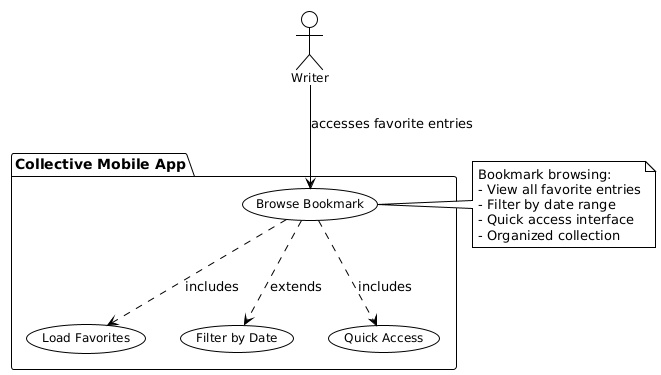
\includegraphics[width=0.8\textwidth]{files/imgs/usecase_U9ojaarlmZ.png}
\caption{Use Case Browse Bookmark}
\label{fig:usecase-browse-bookmark}
\end{figure}

\begin{table}[H]
\centering
\caption{Use Case Browse Bookmark Details}
\label{tab:usecase-browse-bookmark}
\begin{tabular}{|p{3cm}|p{11cm}|}
\hline
\textbf{Use Case ID} & UC-010 \\
\hline
\textbf{Use Case Name} & Browse Bookmark \\
\hline
\textbf{Purpose} & To allow writers to access and browse their bookmarked/favorite entries \\
\hline
\textbf{Role} & Writers \\
\hline
\textbf{Base Scenario} & 1. Writer accesses the favorites/bookmarks section \newline 2. System loads all bookmarked entries \newline 3. System displays entries in chronological or custom order \newline 4. Writer can browse, read, edit, or remove bookmarks \newline 5. Writer can access full entry details and associated media \\
\hline
\textbf{Alternative Scenario} & 1. Writer applies date range filter to bookmarks \newline 2. System filters bookmarked entries by specified dates \newline 3. System displays filtered results \newline OR \newline 1. Writer searches within bookmarked entries \newline 2. System performs search only within favorite entries \newline 3. System displays matching bookmarked entries \\
\hline
\textbf{Exception Scenario} & 1. No bookmarked entries exist - System displays empty state with guidance \newline 2. Bookmark data corrupted - System attempts recovery or resets bookmarks \newline 3. Loading error - System displays retry option \newline 4. Network issues - System shows cached bookmarks with sync status \\
\hline
\end{tabular}
\end{table}

\subsubsection{View Entries}

Figure~\ref{fig:usecase-view-entries} shows the view entries use case diagram. This provides the main interface for browsing all journal entries.

\begin{figure}[H]
\centering
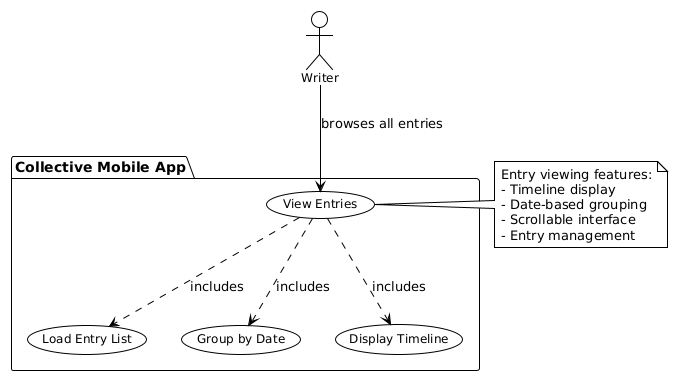
\includegraphics[width=0.8\textwidth]{files/imgs/usecase_U9ojah5omZ.png}
\caption{Use Case View Entries}
\label{fig:usecase-view-entries}
\end{figure}

\begin{table}[H]
\centering
\caption{Use Case View Entries Details}
\label{tab:usecase-view-entries}
\begin{tabular}{|p{3cm}|p{11cm}|}
\hline
\textbf{Use Case ID} & UC-011 \\
\hline
\textbf{Use Case Name} & View Entries \\
\hline
\textbf{Purpose} & To allow writers to browse and view all their journal entries in an organized timeline \\
\hline
\textbf{Role} & Writers \\
\hline
\textbf{Base Scenario} & 1. Writer opens the main journal screen \newline 2. System loads all journal entries from local and cloud storage \newline 3. System groups entries by date for organized display \newline 4. System displays entries in reverse chronological order \newline 5. Writer can scroll through timeline and access individual entries \\
\hline
\textbf{Alternative Scenario} & 1. Writer filters entries by date range \newline 2. System displays entries within specified timeframe \newline OR \newline 1. Writer sorts entries by different criteria (mood, tags, etc.) \newline 2. System reorganizes display according to selected sorting \\
\hline
\textbf{Exception Scenario} & 1. No entries exist - System displays welcome message and entry creation guidance \newline 2. Loading error - System shows cached entries with sync status indicator \newline 3. Large number of entries causes performance issues - System implements pagination \newline 4. Data corruption detected - System attempts recovery and shows error status \\
\hline
\end{tabular}
\end{table}

\subsubsection{Search}

Figure~\ref{fig:usecase-search} shows the search use case diagram. This enables efficient entry discovery through text matching.

\begin{figure}[H]
\centering
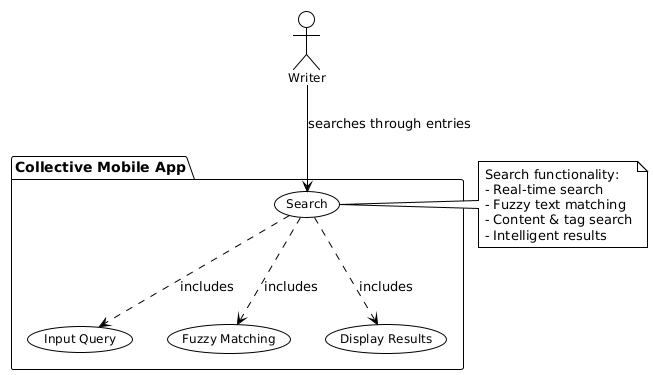
\includegraphics[width=0.8\textwidth]{files/imgs/usecase_U9ojKh5kmZ.png}
\caption{Use Case Search}
\label{fig:usecase-search}
\end{figure}

\begin{table}[H]
\centering
\caption{Use Case Search Details}
\label{tab:usecase-search}
\begin{tabular}{|p{3cm}|p{11cm}|}
\hline
\textbf{Use Case ID} & UC-012 \\
\hline
\textbf{Use Case Name} & Search \\
\hline
\textbf{Purpose} & To allow writers to search through their journal entries using keywords and phrases \\
\hline
\textbf{Role} & Writers \\
\hline
\textbf{Base Scenario} & 1. Writer activates search interface \newline 2. Writer enters search keywords or phrases \newline 3. System performs real-time fuzzy text matching across entry content and tags \newline 4. System displays matching entries with highlighted search terms \newline 5. Writer can access full entries from search results \\
\hline
\textbf{Alternative Scenario} & 1. Writer searches by specific tags \newline 2. System filters entries containing specified tags \newline 3. System displays tag-filtered results \newline OR \newline 1. Writer uses advanced search with multiple criteria \newline 2. System combines text, tag, mood, and date filters \newline 3. System displays comprehensive filtered results \\
\hline
\textbf{Exception Scenario} & 1. No search results found - System displays no results message with search suggestions \newline 2. Search query too short - System requires minimum character count \newline 3. Special characters in search - System sanitizes query and searches \newline 4. Search performance issues - System optimizes query and displays progress indicator \\
\hline
\end{tabular}
\end{table}

\subsubsection{Browse Calendar}

Figure~\ref{fig:usecase-browse-calendar} shows the browse calendar use case diagram. This provides date-based navigation through entries.

\begin{figure}[H]
\centering
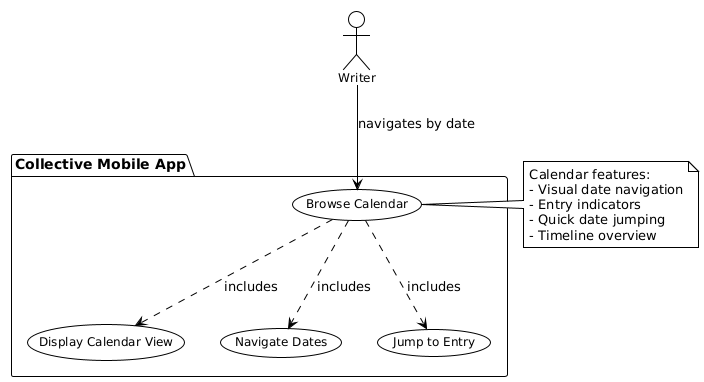
\includegraphics[width=0.8\textwidth]{files/imgs/usecase_U9ojaarFma.png}
\caption{Use Case Browse Calendar}
\label{fig:usecase-browse-calendar}
\end{figure}

\begin{table}[H]
\centering
\caption{Use Case Browse Calendar Details}
\label{tab:usecase-browse-calendar}
\begin{tabular}{|p{3cm}|p{11cm}|}
\hline
\textbf{Use Case ID} & UC-013 \\
\hline
\textbf{Use Case Name} & Browse Calendar \\
\hline
\textbf{Purpose} & To allow writers to navigate their journal entries using a visual calendar interface \\
\hline
\textbf{Role} & Writers \\
\hline
\textbf{Base Scenario} & 1. Writer accesses calendar view from main interface \newline 2. System displays calendar with entry indicators on dates with journal entries \newline 3. Writer navigates through months and years \newline 4. Writer selects specific date with entries \newline 5. System navigates to entries for selected date in main timeline \\
\hline
\textbf{Alternative Scenario} & 1. Writer uses calendar to find entries from specific time period \newline 2. System highlights date ranges with entry activity \newline 3. Writer selects date range for filtered viewing \newline OR \newline 1. Calendar displays mood indicators for each date \newline 2. Writer can visualize emotional patterns over time \newline 3. Writer selects dates based on mood indicators \\
\hline
\textbf{Exception Scenario} & 1. Calendar fails to load - System displays alternative date navigation \newline 2. Date with no entries selected - System offers to create new entry for that date \newline 3. Performance issues with large date ranges - System implements lazy loading \newline 4. Invalid date selection - System corrects to nearest valid date \\
\hline
\end{tabular}
\end{table}

\subsubsection{View Analytics}

Figure~\ref{fig:usecase-view-analytics} shows the view analytics use case diagram. This provides insights into journaling patterns and trends.

\begin{figure}[H]
\centering
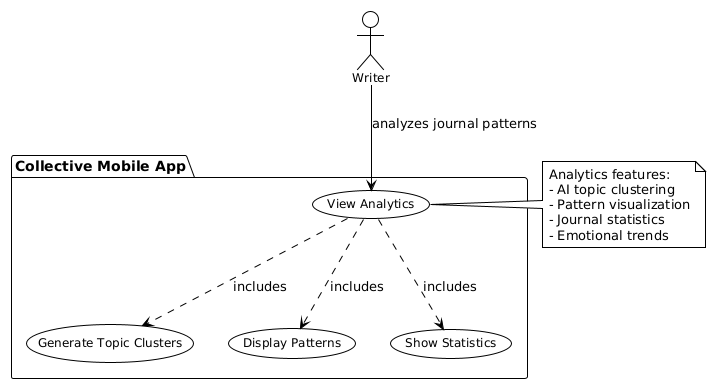
\includegraphics[width=0.8\textwidth]{files/imgs/usecase_U9ojaijEmp.png}
\caption{Use Case View Analytics}
\label{fig:usecase-view-analytics}
\end{figure}

\begin{table}[H]
\centering
\caption{Use Case View Analytics Details}
\label{tab:usecase-view-analytics}
\begin{tabular}{|p{3cm}|p{11cm}|}
\hline
\textbf{Use Case ID} & UC-014 \\
\hline
\textbf{Use Case Name} & View Analytics \\
\hline
\textbf{Purpose} & To allow writers to analyze their journaling patterns, topics, and emotional trends \\
\hline
\textbf{Role} & Writers \\
\hline
\textbf{Base Scenario} & 1. Writer accesses analytics section from main interface \newline 2. System analyzes journal entries to identify topic clusters and patterns \newline 3. System generates visualizations showing topic distribution and trends \newline 4. System displays emotional patterns and mood statistics \newline 5. Writer can explore individual topic clusters and associated entries \\
\hline
\textbf{Alternative Scenario} & 1. System uses cached analytics when available \newline 2. System displays previously generated insights immediately \newline 3. System updates analytics in background when new entries added \newline OR \newline 1. Writer requests analytics refresh \newline 2. System regenerates analysis with current data \newline 3. System displays updated insights and patterns \\
\hline
\textbf{Exception Scenario} & 1. Insufficient data for analytics - System displays message about minimum entry requirements \newline 2. Analytics generation fails - System displays error and retry option \newline 3. Complex analytics take too long - System displays progress and allows backgrounding \newline 4. Analytics data corrupted - System regenerates from source entries \\
\hline
\end{tabular}
\end{table}

\subsubsection{View AI Insights}

Figure~\ref{fig:usecase-view-ai-insights} shows the view AI insights use case diagram. This provides detailed AI-powered analysis of individual entries.

\begin{figure}[H]
\centering
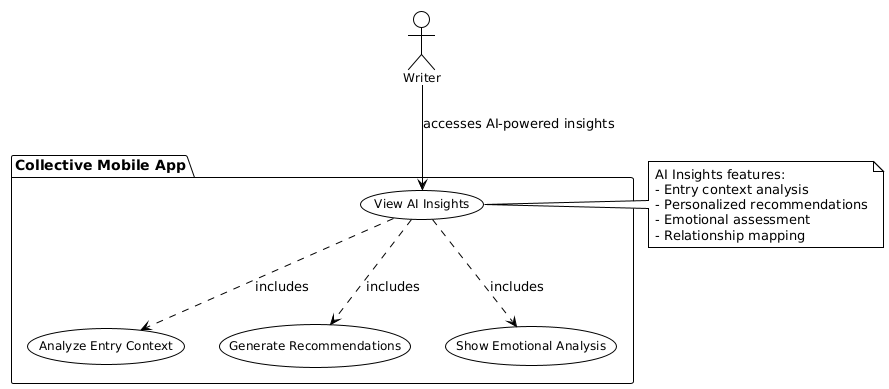
\includegraphics[width=0.8\textwidth]{files/imgs/usecase_U9ojKijEmp.png}
\caption{Use Case View AI Insights}
\label{fig:usecase-view-ai-insights}
\end{figure}

\begin{table}[H]
\centering
\caption{Use Case View AI Insights Details}
\label{tab:usecase-view-ai-insights}
\begin{tabular}{|p{3cm}|p{11cm}|}
\hline
\textbf{Use Case ID} & UC-015 \\
\hline
\textbf{Use Case Name} & View AI Insights \\
\hline
\textbf{Purpose} & To allow writers to access AI-powered insights and analysis for individual journal entries \\
\hline
\textbf{Role} & Writers \\
\hline
\textbf{Base Scenario} & 1. Writer selects AI insights option for a specific entry \newline 2. System analyzes entry content using AI services \newline 3. System generates contextual insights about themes, emotions, and relationships \newline 4. System provides personalized recommendations based on entry content \newline 5. Writer reviews insights and can apply suggestions to future entries \\
\hline
\textbf{Alternative Scenario} & 1. System displays cached insights if previously generated \newline 2. System shows processing status for new analysis \newline 3. System updates insights when analysis completes \newline OR \newline 1. Writer requests insight regeneration \newline 2. System reprocesses entry with updated AI models \newline 3. System displays refreshed insights and recommendations \\
\hline
\textbf{Exception Scenario} & 1. AI service unavailable - System displays cached insights or error message \newline 2. Entry too short for analysis - System suggests minimum content requirements \newline 3. Analysis fails - System provides basic insights and retry option \newline 4. Rate limiting from AI service - System queues analysis for later processing \\
\hline
\end{tabular}
\end{table}

\subsubsection{Manage Offline}

Figure~\ref{fig:usecase-manage-offline} shows the manage offline use case diagram. This ensures functionality without internet connectivity.

\begin{figure}[H]
\centering
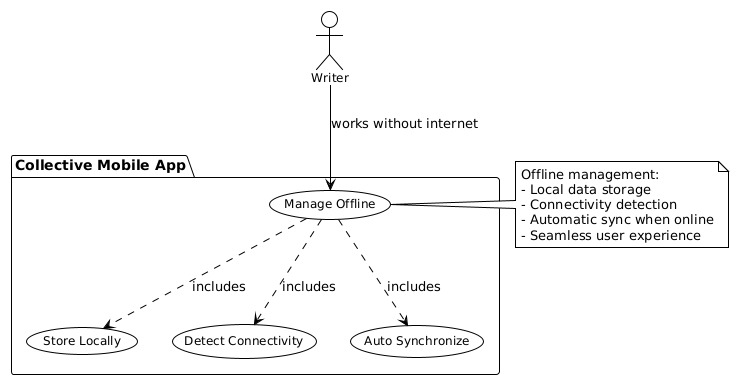
\includegraphics[width=0.8\textwidth]{files/imgs/usecase_U9ojaa5Fma.png}
\caption{Use Case Manage Offline}
\label{fig:usecase-manage-offline}
\end{figure}

\begin{table}[H]
\centering
\caption{Use Case Manage Offline Details}
\label{tab:usecase-manage-offline}
\begin{tabular}{|p{3cm}|p{11cm}|}
\hline
\textbf{Use Case ID} & UC-016 \\
\hline
\textbf{Use Case Name} & Manage Offline \\
\hline
\textbf{Purpose} & To allow writers to use the application fully when internet connectivity is unavailable \\
\hline
\textbf{Role} & Writers \\
\hline
\textbf{Base Scenario} & 1. System detects loss of internet connectivity \newline 2. System switches to offline mode seamlessly \newline 3. System stores all new entries and changes locally \newline 4. System provides full functionality using local database \newline 5. System detects connectivity restoration and synchronizes changes \\
\hline
\textbf{Alternative Scenario} & 1. User manually enables offline mode \newline 2. System prepares for offline operation \newline 3. System caches essential data locally \newline OR \newline 1. Partial connectivity available \newline 2. System optimizes for low-bandwidth operation \newline 3. System prioritizes essential sync operations \\
\hline
\textbf{Exception Scenario} & 1. Local storage insufficient for offline data - System alerts user and suggests cleanup \newline 2. Sync conflicts when connectivity restored - System provides conflict resolution interface \newline 3. Local database corruption - System attempts recovery and alerts user \newline 4. Extended offline period - System optimizes local storage and manages capacity \\
\hline
\end{tabular}
\end{table}

\subsubsection{Generate Analytics}

Figure~\ref{fig:usecase-generate-analytics} shows the generate analytics use case diagram. This backend process creates analytical insights from journal data.

\begin{figure}[H]
\centering
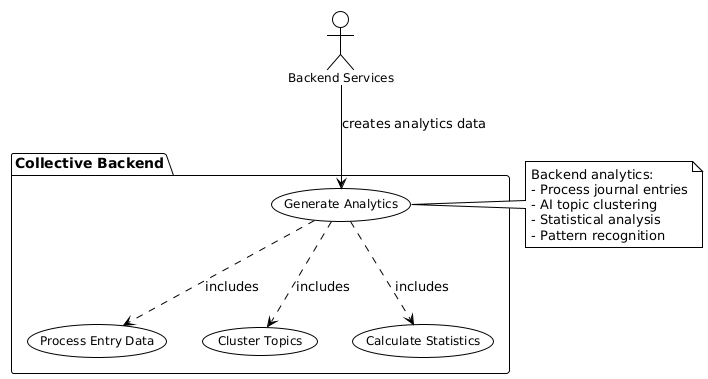
\includegraphics[width=0.8\textwidth]{files/imgs/usecase_U9ojaazhma.png}
\caption{Use Case Generate Analytics}
\label{fig:usecase-generate-analytics}
\end{figure}

\begin{table}[H]
\centering
\caption{Use Case Generate Analytics Details}
\label{tab:usecase-generate-analytics}
\begin{tabular}{|p{3cm}|p{11cm}|}
\hline
\textbf{Use Case ID} & UC-017 \\
\hline
\textbf{Use Case Name} & Generate Analytics \\
\hline
\textbf{Purpose} & To process journal entries and generate analytical insights, patterns, and statistics \\
\hline
\textbf{Role} & Backend Services \\
\hline
\textbf{Base Scenario} & 1. System receives request for analytics generation \newline 2. System processes all available journal entries \newline 3. System applies AI algorithms to identify topic clusters \newline 4. System calculates statistical patterns and trends \newline 5. System stores generated analytics for user access \newline 6. System caches results for improved performance \\
\hline
\textbf{Alternative Scenario} & 1. System performs incremental analytics update \newline 2. System processes only new entries since last analysis \newline 3. System updates existing analytics with new patterns \newline OR \newline 1. System runs scheduled background analytics \newline 2. System automatically updates insights for active users \newline 3. System optimizes processing for system resources \\
\hline
\textbf{Exception Scenario} & 1. Insufficient data for meaningful analytics - System provides guidance on minimum requirements \newline 2. Processing timeout due to large dataset - System implements chunked processing \newline 3. AI service unavailable - System falls back to basic statistical analysis \newline 4. Memory or processing constraints - System optimizes algorithms and processes in batches \\
\hline
\end{tabular}
\end{table}

\subsubsection{Generate Insights}

Figure~\ref{fig:usecase-generate-insights} shows the generate insights use case diagram. This backend process creates personalized AI insights for individual entries.

\begin{figure}[H]
\centering
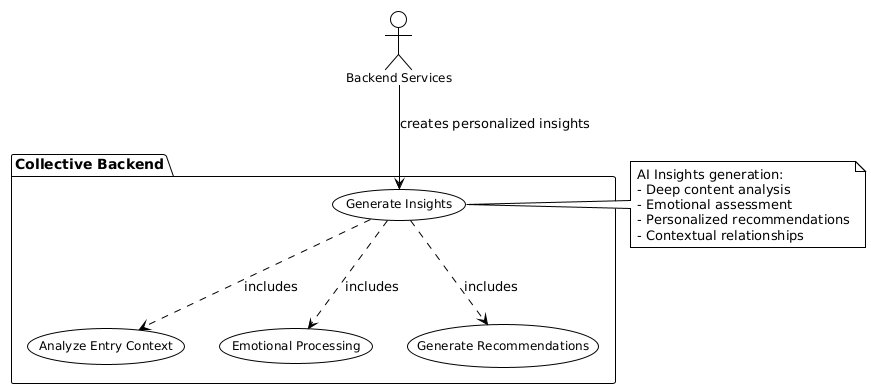
\includegraphics[width=0.8\textwidth]{files/imgs/usecase_U9ojKijkmZ.png}
\caption{Use Case Generate Insights}
\label{fig:usecase-generate-insights}
\end{figure}

\begin{table}[H]
\centering
\caption{Use Case Generate Insights Details}
\label{tab:usecase-generate-insights}
\begin{tabular}{|p{3cm}|p{11cm}|}
\hline
\textbf{Use Case ID} & UC-018 \\
\hline
\textbf{Use Case Name} & Generate Insights \\
\hline
\textbf{Purpose} & To create personalized AI-powered insights and recommendations for individual journal entries \\
\hline
\textbf{Role} & Backend Services \\
\hline
\textbf{Base Scenario} & 1. System receives request for entry-specific insight generation \newline 2. System analyzes entry content using natural language processing \newline 3. System performs emotional and contextual analysis \newline 4. System generates personalized recommendations and insights \newline 5. System stores insights linked to specific entry \newline 6. System provides insights to user interface \\
\hline
\textbf{Alternative Scenario} & 1. System uses historical user data to enhance insights \newline 2. System considers user's journaling patterns and preferences \newline 3. System provides more personalized and relevant recommendations \newline OR \newline 1. System batches multiple entries for efficient processing \newline 2. System generates insights for multiple entries simultaneously \newline 3. System optimizes AI service usage and costs \\
\hline
\textbf{Exception Scenario} & 1. AI service rate limiting - System queues requests and processes when capacity available \newline 2. Entry content insufficient for analysis - System provides general insights and suggestions \newline 3. Processing failure - System logs error and provides retry mechanism \newline 4. User privacy restrictions - System processes locally or uses anonymized analysis \\
\hline
\end{tabular}
\end{table}

\subsection{Product Functions}\label{subsec:productFunctions}

This section presents a comprehensive overview of the functional requirements for the \textbf{Collective} mobile journaling application. Each function is detailed with a unique identifier, feature name, description, and accessible user role. The functions are organized by categories covering authentication, journaling core features, content management, AI-powered features, and system utilities. Table~\ref{tab:function-summary} provides an overview of all 31 functional requirements.

\begin{table}[H]
\centering
\caption{Functional Requirements Summary}
\label{tab:function-summary}
\begin{tabular}{|p{2.5cm}|p{3cm}|p{7.5cm}|}
\hline
\textbf{Category} & \textbf{Function Range} & \textbf{Description} \\
\hline
Authentication & F001 - F003 & User registration, login, and logout functionality \\
\hline
Core Journaling & F004 - F007 & Entry creation, editing, deletion, and submission \\
\hline
Content Enhancement & F008 - F011 & Mood setting, tagging, media attachment, bookmarking \\
\hline
Content Management & F012 - F015 & Entry viewing, searching, calendar browsing, bookmark management \\
\hline
AI Analysis & F016 - F019 & AI insights generation and analytics viewing \\
\hline
Data Management & F020 - F023 & Data storage, retrieval, offline management, synchronization \\
\hline
User Interface & F024 - F027 & Selection modes, themes, responsive design, progress feedback \\
\hline
System Utilities & F028 - F031 & Error handling, validation, performance, security \\
\hline
\end{tabular}
\end{table}

\newpage

\subsubsection{Authentication and User Management Functions}

The authentication system provides secure user access control with multiple authentication methods. These functions ensure user identity verification and session management.

\begin{table}[H]
\centering
\caption{Authentication Functions}
\label{tab:auth-functions}
\begin{tabular}{|p{0.8cm}|p{2.2cm}|p{9.5cm}|p{1.5cm}|}
\hline
\textbf{ID} & \textbf{Function} & \textbf{Description} & \textbf{Role} \\
\hline
F001 & Register & Allow new users to create accounts using email/password, Google OAuth, or Twitter/X OAuth with validation and secure profile creation & Writer \\
\hline
F002 & Login & Enable existing users to authenticate through email/password or OAuth providers with credential validation and interface redirection & Writer \\
\hline
F003 & Logout & Allow users to securely terminate sessions, clear authentication data, and return to login screen & Writer \\
\hline
\end{tabular}
\end{table}

\subsubsection{Core Journaling Functions}

\begin{table}[H]
\centering
\caption{Core Journaling Functions}
\label{tab:core-journaling-functions}
\begin{tabular}{|p{0.8cm}|p{2.2cm}|p{9.5cm}|p{1.5cm}|}
\hline
\textbf{ID} & \textbf{Function} & \textbf{Description} & \textbf{Role} \\
\hline
F004 & Write Entry & Provide minimalist, distraction-free writing interface with text composition, automatic word count tracking, real-time editing, auto-save functionality, and maintained writing focus & Writer \\
\hline
F005 & Submit Entry & Allow users to finalize and save completed entries with content validation, immediate local database storage, cloud synchronization queueing, and visual save confirmation & Writer \\
\hline
F006 & Edit Entry & Enable modification of existing journal entries while preserving original timestamps, tracking edit history, supporting text/mood/media modifications, and maintaining data integrity & Writer \\
\hline
F007 & Delete Entry & Enable removal of unwanted journal entries with confirmation dialogs, permanent deletion from local and cloud storage, and updated entry statistics & Writer \\
\hline
\end{tabular}
\end{table}

\newpage

\subsubsection{Content Enhancement Functions}

\begin{table}[H]
\centering
\caption{Content Enhancement Functions - Part 1}
\label{tab:content-enhancement-functions-1}
\begin{tabular}{|p{0.8cm}|p{2.2cm}|p{9.5cm}|p{1.5cm}|}
\hline
\textbf{Feature ID} & \textbf{Feature} & \textbf{Description} & \textbf{Accessible Role} \\
\hline
F008 & Set Mood & Allow users to associate emotional states with entries using predefined mood options with emoji representations, enabling mood selection during or after entry creation for emotional pattern tracking & Writer \\
\hline
F009 & Append Tags & Enable manual categorization of journal entries with custom tag creation, AI-powered tag suggestions based on content, thematic organization, and efficient search facilitation & Writer \\
\hline
\end{tabular}
\end{table}

\begin{table}[H]
\centering
\caption{Content Enhancement Functions - Part 2}
\label{tab:content-enhancement-functions-2}
\begin{tabular}{|p{0.8cm}|p{2.2cm}|p{9.5cm}|p{1.5cm}|}
\hline
\textbf{Feature ID} & \textbf{Feature} & \textbf{Description} & \textbf{Accessible Role} \\
\hline
F010 & Attach Media & Support image attachment from device gallery, direct photo capture, automatic compression for storage efficiency, local and cloud storage management, and media display within entries & Writer \\
\hline
F011 & Set Bookmark & Allow marking of important entries for quick access with visual indicators, bookmark management, and organized favorites collection & Writer \\
\hline
\end{tabular}
\end{table}

\subsubsection{Content Management and Retrieval Functions}

\begin{table}[H]
\centering
\caption{Content Management and Retrieval Functions - Part 1}
\label{tab:content-management-functions-1}
\begin{tabular}{|p{0.8cm}|p{2.2cm}|p{9.5cm}|p{1.5cm}|}
\hline
\textbf{Feature ID} & \textbf{Feature} & \textbf{Description} & \textbf{Accessible Role} \\
\hline
F012 & View Entries & Display all journal entries in chronological order with date grouping, infinite scrolling for large collections, entry previews with timestamps and metadata, and bulk operation support & Writer \\
\hline
F013 & Search Entries & Enable text-based search across all entry content with fuzzy search capability, tag and metadata searching, real-time results, and search term highlighting & Writer \\
\hline
\end{tabular}
\end{table}

\begin{table}[H]
\centering
\caption{Content Management and Retrieval Functions - Part 2}
\label{tab:content-management-functions-2}
\begin{tabular}{|p{0.8cm}|p{2.2cm}|p{9.5cm}|p{1.5cm}|}
\hline
\textbf{Feature ID} & \textbf{Feature} & \textbf{Description} & \textbf{Accessible Role} \\
\hline
F014 & Browse Calendar & Display entries organized by calendar dates with visual indicators for entry days, quick date navigation, entry count tracking, and date range filtering & Writer \\
\hline
F015 & Browse Bookmarks & Display all bookmarked entries in dedicated view with quick access to important content, bookmark organization, and removal capabilities & Writer \\
\hline
\end{tabular}
\end{table}

\newpage

\subsubsection{AI-Powered Analysis Functions}

\begin{table}[H]
\centering
\caption{AI-Powered Analysis Functions}
\label{tab:ai-analysis-functions}
\begin{tabular}{|p{0.8cm}|p{2.2cm}|p{9.5cm}|p{1.5cm}|}
\hline
\textbf{Feature ID} & \textbf{Feature} & \textbf{Description} & \textbf{Accessible Role} \\
\hline
F016 & Generate Insights & Create personalized AI-powered insights for individual entries using natural language processing, emotional and contextual analysis, personalized recommendations, and entry-specific pattern identification & Backend Services \\
\hline
F017 & View AI Insights & Display AI-generated insights for individual entries with detailed content analysis, emotional patterns, thematic connections, personalized recommendations, and sharing capabilities & Writer \\
\hline
F018 & Generate Analytics & Process journal entries for analytical insights, identify topic clusters and thematic patterns, calculate statistical trends, generate emotional tracking, and provide comprehensive behavior analytics & Backend Services \\
\hline
F019 & View Analytics & Display comprehensive analytics dashboard with topic clusters, content distribution, emotional trends, mood statistics, journaling pattern visualization, and topic area exploration & Writer \\
\hline
\end{tabular}
\end{table}

\subsubsection{Data Management and Synchronization Functions}

\begin{table}[H]
\centering
\caption{Data Management and Synchronization Functions - Part 1}
\label{tab:data-management-functions-1}
\begin{tabular}{|p{0.8cm}|p{2.2cm}|p{9.5cm}|p{1.5cm}|}
\hline
\textbf{Feature ID} & \textbf{Feature} & \textbf{Description} & \textbf{Accessible Role} \\
\hline
F020 & Store Entries & Securely store journal entries in local database with data integrity maintenance, immediate storage for offline capability, sensitive data encryption, and storage optimization & Backend Services \\
\hline
F021 & Retrieve Entries & Efficiently load journal entries from storage with fast retrieval for optimal performance, large dataset pagination, session consistency, and data recovery mechanisms & Backend Services \\
\hline
\end{tabular}
\end{table}

\begin{table}[H]
\centering
\caption{Data Management and Synchronization Functions - Part 2}
\label{tab:data-management-functions-2}
\begin{tabular}{|p{0.8cm}|p{2.2cm}|p{9.5cm}|p{1.5cm}|}
\hline
\textbf{Feature ID} & \textbf{Feature} & \textbf{Description} & \textbf{Accessible Role} \\
\hline
F022 & Manage Offline & Enable full functionality without internet connectivity through automatic detection, local action storage, seamless offline-to-online transitions, and synchronization integrity & Backend Services \\
\hline
F023 & Cloud Synchronization & Synchronize local data with Firebase cloud storage including conflict resolution, incremental sync for bandwidth efficiency, multi-device consistency, and automatic/manual sync triggers & Backend Services \\
\hline
\end{tabular}
\end{table}

\subsubsection{User Interface and System Functions}

\begin{table}[H]
\centering
\caption{User Interface and Experience Functions}
\label{tab:ui-ux-functions}
\begin{tabular}{|p{0.8cm}|p{2.2cm}|p{9.5cm}|p{1.5cm}|}
\hline
\textbf{Feature ID} & \textbf{Feature} & \textbf{Description} & \textbf{Accessible Role} \\
\hline
F024 & Selection Mode & Enable multi-entry selection for bulk operations with visual feedback, batch deletion, date range selection, and maintained selection state during navigation & Writer \\
\hline
F025 & Theme Management & Provide automatic light/dark theme switching responding to system preferences with consistent visual design, readability optimization, and accessibility support & Writer \\
\hline
F026 & Responsive Design & Adapt interface layout to different screen sizes with device orientation support, optimized touch targets, consistent cross-platform experience, and accessibility features & Writer \\
\hline
F027 & Progress Feedback & Provide visual indicators for ongoing operations including sync status, connectivity information, loading states, completion confirmations, and system status indicators & Writer \\
\hline
\end{tabular}
\end{table}

\newpage

\begin{table}[H]
\centering
\caption{System Utility Functions}
\label{tab:system-utility-functions}
\begin{tabular}{|p{0.8cm}|p{2.2cm}|p{9.5cm}|p{1.5cm}|}
\hline
\textbf{Feature ID} & \textbf{Feature} & \textbf{Description} & \textbf{Accessible Role} \\
\hline
F028 & Error Handling & Gracefully handle system errors and exceptions with meaningful user messages, automatic recovery mechanisms, debugging logs, and application stability maintenance & Backend Services \\
\hline
F029 & Data Validation & Validate user input for data integrity, enforce business rules and constraints, prevent malformed data entry, provide immediate validation feedback, and maintain data quality & Backend Services \\
\hline
F030 & Performance Optimization & Optimize application performance for mobile devices with efficient data loading, caching strategies, battery/memory usage minimization, smooth animations, and responsive interactions & Backend Services \\
\hline
F031 & Security Management & Implement secure authentication and authorization, encrypt sensitive data at rest and in transit, protect against vulnerabilities, manage privacy compliance, and secure API communications & Backend Services \\
\hline
\end{tabular}
\end{table}

These 31 functional requirements collectively form the comprehensive feature set of the \textbf{Collective} mobile journaling application, ensuring a complete and user-friendly journaling experience while maintaining the simplicity and focus that distinguishes the application from traditional digital journaling platforms.

\section{Construction}\label{sec:construction}

In this phase, the system development and implementation tasks are focused, which include system developing, programming, and testing. The Collective mobile journaling application prototype is developed using Flutter framework with Firebase backend integration to gain feedback from users and improve the system functionality.

The development process follows agile principles with iterative development cycles. Key implementation activities include:

\begin{itemize}
\item Frontend development using Flutter with Material Design 3
\item Backend integration with Firebase Authentication and Firestore
\item AI service integration with DeepSeek API for entry analysis
\item Local database implementation using Sembast for offline functionality
\item User interface testing and optimization for mobile devices
\item Performance optimization and security implementation
\end{itemize}

The construction phase emphasizes rapid prototyping and continuous user feedback integration to ensure the application meets user expectations and maintains the simplicity that distinguishes it from traditional digital journaling platforms.

\section{Cutover}\label{sec:cutover}

In this phase, the installation and deployment of the Collective mobile journaling system is conducted where necessary user acceptance testing and user training take place. This ensures that no faults or mistakes occur in the system and that it meets all requirements and objectives as expected.

The cutover phase includes deployment preparation, user acceptance testing with target users, performance validation on various mobile devices, and final system optimization based on user feedback.

\subsection{Project Resources}\label{subsec:projectResources}

\subsubsection{Resource List}

Table~\ref{tab:resource-list} presents the comprehensive list of software tools and technologies used in the development of the Collective mobile journaling application.

\begin{table}[H]
\centering
\caption{Project Resource List}
\label{tab:resource-list}
\begin{tabular}{|p{3.5cm}|p{6cm}|p{3.5cm}|}
\hline
\textbf{SOFTWARE REQUIREMENT} & \textbf{Description} & \textbf{Total Cost} \\
\hline
Flutter SDK & Mobile application development framework & RM 0.00 \\
\hline
Android Studio & IDE for Android development and debugging & RM 0.00 \\
\hline
Visual Studio Code & Code editor for development & RM 0.00 \\
\hline
Firebase Console & Backend services and cloud storage & RM 0.00 \\
\hline
DeepSeek API & AI service for journal analysis & RM 0.00 \\
\hline
Google Chrome & Testing and research & RM 0.00 \\
\hline
Microsoft Word & Documentation and reporting & RM 0.00 \\
\hline
Microsoft Excel & Project planning and data analysis & RM 0.00 \\
\hline
LaTeX & Thesis documentation & RM 0.00 \\
\hline
PlantUML & UML diagram generation & RM 0.00 \\
\hline
Figma & UI/UX design and prototyping & RM 0.00 \\
\hline
Git & Version control system & RM 0.00 \\
\hline
\textbf{Total} & & \textbf{RM 0.00} \\
\hline
\end{tabular}
\end{table}

\subsection{Conclusion}\label{subsec:methodologyConclusion}

This chapter presents the comprehensive research methodology for the Collective mobile journaling application using the Rapid Application Development (RAD) approach. The methodology encompasses requirement planning, user design, construction, and cutover phases, ensuring systematic development that prioritizes user feedback and iterative improvement.

Understanding the application requirements from the user's perspective through detailed use case analysis, activity flows, and functional specifications enables the development of a user-friendly application that bridges traditional and digital journaling experiences. The RAD methodology's emphasis on rapid prototyping and continuous user involvement ensures that the final application meets user expectations while maintaining the simplicity and focus that distinguishes Collective from existing digital journaling platforms.
